%File: less_is_more_aaai.tex
%
% AAAI 2026 TEMPLATE for "Less is More" Paper
% For ANONYMOUS SUBMISSION: uncomment the next line
\def\aaaianonymous{true}
%
% For CAMERA-READY VERSION: comment out or delete the next line
% \def\aaaianonymous{true}
%
%%%%%%%%%%%%%%%%%%%%%%%%%%%%%%%%%%%%%%%%%%%%%%%%%%%%%%%%%%%%%%%%%%%%%%%

\documentclass[letterpaper]{article} % DO NOT CHANGE THIS

% Conditional package loading based on version
\ifdefined\aaaianonymous
    \usepackage[submission]{aaai2026}  % Anonymous submission version
\else
    \usepackage{aaai2026}              % Camera-ready version
\fi

\usepackage{times}  % DO NOT CHANGE THIS
\usepackage{helvet}  % DO NOT CHANGE THIS
\usepackage{courier}  % DO NOT CHANGE THIS
\usepackage[hyphens]{url}  % DO NOT CHANGE THIS
\usepackage{graphicx} % DO NOT CHANGE THIS
\urlstyle{rm} % DO NOT CHANGE THIS
\def\UrlFont{\rm}  % DO NOT CHANGE THIS
\usepackage{natbib}  % DO NOT CHANGE THIS AND DO NOT ADD ANY OPTIONS TO IT
\usepackage{caption} % DO NOT CHANGE THIS AND DO NOT ADD ANY OPTIONS TO IT
\frenchspacing  % DO NOT CHANGE THIS
\setlength{\pdfpagewidth}{8.5in} % DO NOT CHANGE THIS
\setlength{\pdfpageheight}{11in} % DO NOT CHANGE THIS

% Additional packages for tables and math
\usepackage{booktabs}
\usepackage{multirow}
\usepackage{amsmath}

%
% Keep the \pdfinfo as shown here. There's no need
% for you to add the /Title and /Author tags.
\pdfinfo{
/TemplateVersion (2026.1)
}

\setcounter{secnumdepth}{0} %May be changed to 1 or 2 if section numbers are desired.

% Title - conditionally set based on version
\ifdefined\aaaianonymous
    \title{Less is More: Simple Linear Fusion Outperforms Complex Retrieval-Augmented Generation Systems}
\else
    \title{Less is More: Simple Linear Fusion Outperforms Complex Retrieval-Augmented Generation Systems}
\fi

% Author and affiliation information
\ifdefined\aaaianonymous
\author{
    Anonymous Submission
}
\affiliations{
    Anonymous Institution\\
    Anonymous Address\\
    anonymous@email.com
}
\else
\author{
    % Authors will be filled in camera-ready version
    Author Name\textsuperscript{\rm 1}
}
\affiliations{
    % Affiliations will be filled in camera-ready version
    \textsuperscript{\rm 1}Institution Name\\
    Address Line 1\\
    Address Line 2\\
    email@institution.edu
}
\fi

\begin{document}

\maketitle

\begin{abstract}
In information retrieval, multi-retriever fusion has become an important technique for improving retrieval performance. The conventional wisdom suggests that more complex fusion strategies yield better results, prompting researchers to develop increasingly sophisticated methods. However, our research challenges this assumption by proposing a "Less is More" perspective.

Our experimental results reveal an interesting finding: \textbf{under the specific datasets and experimental conditions of this study, simple linear fusion methods can in certain cases achieve or exceed the performance of complex methods}. Specifically, simple linear fusion outperforms the standard RRF method by 8.2\%, 7.2\%, and 10.9\% in MRR performance on FIQA, Quora, and SciDocs datasets respectively, with a 2.2\% improvement on SciFact dataset. Importantly, ablation experiments show that removing complex components (such as query analyzers) can improve performance in certain cases. Additionally, simple methods have significant advantages in computational efficiency, with inference speed significantly faster than complex methods.

These findings provide empirical support in specific scenarios for the hypothesis that "simple methods may be more effective," questioning the prevalent assumption that "complexity equals better," and providing important reference principles for practical system design.
\end{abstract}

% Links section - only shown in camera-ready version
\ifdefined\aaaianonymous
% For anonymous submissions, do not include links that could reveal identity
\else
\begin{links}
    \link{Code}{https://github.com/anonymous/less-is-more-rag}
    \link{Datasets}{https://github.com/anonymous/less-is-more-data}
\end{links}
\fi

\section{Introduction}

With the development of large language models and Retrieval-Augmented Generation (RAG) technology \cite{lewis2020retrieval}, multi-retriever fusion has become an important research direction in information retrieval. In recent years, RAG technology has rapidly evolved from basic retrieval-generation architectures to more complex multimodal \cite{chen2022multimodal} and agent-based systems \cite{singh2025agentic}, with the latest survey studies \cite{gao2024retrieval} systematically reviewing the development trajectory and future directions of RAG technology. Multi-retriever systems improve retrieval performance by combining different types of retrievers (such as dense vector retrieval \cite{karpukhin2020dense} and sparse BM25 retrieval \cite{robertson2009probabilistic}), but how to effectively fuse the results of multiple retrievers has become a key challenge.

\subsection{Research Background and Motivation}

\textbf{From Practical Needs to Theoretical Discovery}

This research stems from our practical experience in building production-level multi-retriever fusion systems. Inspired by the numerous complex fusion strategies proposed by the academic community in recent years, we conducted a systematic analysis of recent papers and identified several major innovation directions:

\begin{enumerate}
\item \textbf{Query Analysis and Classification}: Such as query decomposition proposed by LevelRAG \cite{jiang2023levelrag} and complexity classification by Adaptive-RAG \cite{jeong2024adaptive}
\item \textbf{Dynamic Weight Adjustment}: Mechanisms that dynamically adjust fusion weights based on query features
\item \textbf{Adaptive Routing Strategies}: Such as the parameter adaptive system of HyPA-RAG \cite{su2024hypa}
\item \textbf{Knowledge Graph Enhancement}: Such as structured knowledge integration of KG-Infused RAG \cite{edge2024kg}
\end{enumerate}

Based on these advanced concepts, we built a complete system architecture containing query analyzers, adaptive routers, and dynamic fusion engines (detailed in Section 3), expecting to significantly improve retrieval performance by increasing system complexity. Our initial hypothesis was that more complex adaptive mechanisms could intelligently select optimal fusion strategies based on query features, thereby outperforming simple static methods.

\subsection{Unexpected Discovery and Research Contribution}

\textbf{Challenging Initial Assumptions with Experimental Findings}

However, in systematic experimental evaluation on 6 BEIR datasets \cite{thakur2021beir}, we obtained an important finding: \textbf{under our experimental conditions, simple linear fusion methods performed better than our designed complex adaptive system on most datasets}.

This finding completely overturned our initial assumptions. We originally expected the query analyzer to accurately identify query types, the adaptive router to intelligently select optimal strategies, and the dynamic fusion engine to adjust weights based on context. But experimental results showed that these complex components not only failed to improve performance, but in some cases even had negative effects.

\textbf{Quantified Performance Comparison Results}:

\begin{itemize}
\item Simple linear fusion outperformed standard RRF by 8.2\%, 7.2\%, and 10.9\% on FIQA, Quora, and SciDocs datasets respectively, with a 2.2\% improvement on SciFact dataset
\item Ablation experiments revealed an even more noteworthy phenomenon: gradually removing complex components (such as query analyzers and adaptive routers) not only did not degrade performance, but even brought 10.9\% performance improvement on SciDocs dataset
\item Computational efficiency analysis showed that simple methods have significant advantages in inference speed, while complex adaptive systems have significantly higher computational overhead
\end{itemize}

These findings under specific experimental conditions challenge our initial design philosophy, and more importantly question the prevalent assumption of "complexity equals better" in the information retrieval field, providing empirical support for the "Less is More" design philosophy.

\textbf{Main Contributions of This Paper}:

\begin{enumerate}
\item \textbf{Real System-Driven Research}: Based on complete production-level multi-retriever system development experience, providing a complete research path from complex design to simple effectiveness
\item \textbf{Systematic Empirical Validation}: Implemented and evaluated 8 fusion strategies on 6 BEIR datasets, revealing performance differences between simple and complex methods through rigorous comparative experiments
\item \textbf{Counter-Intuitive Important Findings}: Proved that in multi-retriever fusion tasks, simple linear methods can not only achieve, but often exceed the performance of carefully designed complex adaptive methods
\item \textbf{In-Depth Complexity Analysis}: Through detailed ablation experiments and efficiency analysis, revealed the negative impacts that complex components may have, including error propagation, overfitting, and computational overhead
\item \textbf{Practical Guidance Value}: Based on real system development and experimental results, provided specific strategy selection guidance and "simplicity first" design principles for practical retrieval system design
\end{enumerate}

\subsection{Fusion Method Complexity Classification}

To clearly distinguish fusion methods of different complexity levels, we established classification criteria based on the following four dimensions:

\begin{enumerate}
\item \textbf{Parameter Complexity}: Number of parameters and tuning difficulty
\item \textbf{Computational Complexity}: Algorithm time complexity and computational requirements
\item \textbf{System Architecture}: Number of required components and coordination complexity
\item \textbf{Training Requirements}: Whether complex learning or optimization processes are needed
\end{enumerate}

Based on these classification criteria, we categorize fusion methods into three classes:
\begin{itemize}
\item \textbf{Simple Methods}: Linear weighted fusion, max score fusion, etc., with few parameters and simple computation
\item \textbf{Medium Complexity Methods}: RRF, etc., with certain mathematical foundation but relatively simple implementation
\item \textbf{Complex Methods}: Adaptive fusion, LLM-based dynamic weight adjustment, etc., requiring coordination of multiple subsystems
\end{itemize}

\section{Related Work}

\subsection{Multi-Retriever Fusion Methods}

Multi-retriever fusion has been extensively studied in information retrieval. Traditional approaches include Reciprocal Rank Fusion (RRF) \cite{cormack2009reciprocal}, which combines rankings from different retrievers using reciprocal rank scores. Recent work has explored more sophisticated fusion strategies, including learning-to-rank approaches \cite{liu2009learning} and neural fusion methods \cite{zamani2018neural}.

\subsection{Retrieval-Augmented Generation}

RAG systems have gained significant attention with the rise of large language models \cite{lewis2020retrieval}. Recent surveys \cite{gao2024retrieval} provide comprehensive overviews of RAG architectures and applications. Multi-modal RAG systems \cite{chen2022multimodal} and agent-based approaches \cite{singh2025agentic} represent the latest developments in this field.

\subsection{Query Analysis and Adaptive Routing}

Query analysis and routing represent another class of methods for improving retrieval performance by analyzing query characteristics to select the most appropriate retrieval strategies. Recent developments in agentic RAG systems \cite{singh2025agentic} have brought new perspectives to query routing by introducing agent-based planning and decision-making capabilities to optimize the retrieval process.

\subsubsection{Query Decomposition and Rewriting}

LevelRAG \cite{jiang2023levelrag} proposed a hierarchical architecture that uses high-level searchers to decompose complex queries into atomic queries, which are then optimized by low-level searchers. This method is particularly suitable for multi-hop reasoning tasks but has high system complexity requiring coordination of multiple components.

\subsubsection{Query Complexity Classification}

Adaptive-RAG \cite{jeong2024adaptive} proposed a classification method based on query complexity, categorizing queries into simple, medium, and complex classes, and selecting different retrieval strategies for each class. This method embodies the idea of adaptive processing based on query characteristics, but accurate classification of query complexity remains a challenge.

\subsubsection{Adaptive Routing Strategies}

Self-RAG \cite{jeong2024adaptive} and similar works proposed routing mechanisms based on model self-reflection, dynamically deciding when to retrieve and what content to retrieve. These methods increase system flexibility but also significantly increase computational complexity and implementation difficulty.

\section{Methodology}

This section details the complete multi-retriever fusion system we built and the various fusion strategies implemented and evaluated. We will first present the overall system architecture design, then introduce the selection and configuration of basic retrievers, followed by detailed descriptions of implementation details from simple linear fusion to complex adaptive methods, and finally analyze their theoretical foundations and computational complexity.

\subsection{System Architecture Design}

\textbf{Complete Multi-Retriever Fusion System}

To systematically compare the performance of different fusion strategies, we built a complete retrieval system containing multiple components. The system's design philosophy is to support various fusion strategies from simple to complex through a modular approach, ensuring fairness in experimental comparisons.

\textbf{System Core Components}:

\begin{enumerate}
\item \textbf{Diversified Retriever Module}: Contains 6 different types of retrievers (BM25, dense retriever, graph retriever, efficient vector index, semantic enhanced BM25, and cascade retriever), providing diverse retrieval results for fusion

\item \textbf{Query Analyzer}: Responsible for analyzing query features, classifying queries into entity queries, keyword queries, and semantic queries, providing decision basis for adaptive fusion

\item \textbf{Adaptive Router}: Dynamically selects optimal retriever combinations and fusion strategies based on query analysis results, implementing intelligent retrieval routing

\item \textbf{Multi-Strategy Fusion Engine}: Supports 8 different fusion strategies, from simple linear weighting to complex adaptive weight adjustment

\item \textbf{Evaluation and Monitoring Module}: Provides comprehensive performance evaluation and system monitoring functions, supporting real-time strategy effectiveness analysis
\end{enumerate}

\textbf{Design Intent and Expectations}:

Our intention in building this complex system was to expect significant retrieval performance improvements through intelligent query analysis, adaptive routing decisions, and dynamic fusion weight adjustment. We hypothesized that system complexity could bring corresponding performance benefits, especially in automatically selecting optimal strategies when processing different types of queries.

However, as subsequent experimental results show, the actual performance of this complex system formed a sharp contrast with our expectations, leading to deep thinking about the "relationship between complexity and performance."

\subsection{Basic Retrievers}

\textbf{Main Retriever Configuration}

Although our system supports 6 different retrievers, to ensure consistency in experimental comparisons and interpretability of results, we mainly use two complementary retrievers in fusion strategy comparison experiments. This choice is based on their complementarity on different types of queries and stable performance in BEIR benchmark tests. This design philosophy is consistent with the collaborative working principles of multi-retriever emphasized in recent RAG system research \cite{gao2024retrieval}, improving overall retrieval performance by combining the advantages of sparse and dense retrievers.

\subsubsection{Sparse Retriever (BM25)}

We use the BM25 algorithm as the sparse retriever with standard parameters ($k_1 = 1.2$, $b = 0.75$), which provides excellent exact keyword matching capabilities.

\subsubsection{Dense Retriever (E5-large-v2)}

For dense retrieval, we use the E5-large-v2 model \cite{wang2022text}, which provides 1024-dimensional embeddings and excels at semantic matching tasks.

\subsubsection{Retriever Complementarity Analysis}

The combination of BM25 and E5-large-v2 provides good complementarity:

\begin{itemize}
\item \textbf{Query Type Coverage}: BM25 excels at keyword queries, while E5-large-v2 performs better on semantic queries
\item \textbf{Matching Mechanism}: BM25 uses exact term matching, while E5-large-v2 uses semantic similarity
\item \textbf{Failure Mode Diversity}: Different retrievers fail on different types of queries, providing robustness through fusion
\end{itemize}

\subsection{Fusion Strategy Detailed Design}

\textbf{Strategy Spectrum from Simple to Complex}

We implemented and evaluated 8 fusion strategies in our system, from the simplest linear weighting to the most complex adaptive fusion, covering current mainstream fusion methods. Each strategy has its specific design philosophy and applicable scenarios. Our design draws from traditional fusion method ideas while also referencing innovative methods like RAG-Fusion \cite{rackauckas2024rag}.

\textbf{Experimental Design Philosophy}: Our goal is to verify our initial hypothesis through systematic comparative experiments—complex adaptive strategies should outperform simple static methods. To this end, we carefully designed a strategy gradient from simple to complex, expecting to observe performance improvements with increasing complexity.

\subsubsection{Simple Fusion Strategies}

\textbf{1. Linear Equal Weight (Linear Equal)}

The simplest fusion method using equal weights:
$$\text{score}(d) = 0.5 \times \text{score}_{\text{BM25}}(d) + 0.5 \times \text{score}_{\text{dense}}(d)$$

\textbf{2. Linear BM25-Dominant (Linear BM25-Dom)}

Linear fusion favoring BM25:
$$\text{score}(d) = 0.7 \times \text{score}_{\text{BM25}}(d) + 0.3 \times \text{score}_{\text{dense}}(d)$$

\textbf{3. Linear Vector-Dominant (Linear Vector-Dom)}

Linear fusion favoring dense retrieval:
$$\text{score}(d) = 0.3 \times \text{score}_{\text{BM25}}(d) + 0.7 \times \text{score}_{\text{dense}}(d)$$

\textbf{4. Max Score Fusion (Max Score)}

Takes the maximum score from both retrievers:
$$\text{score}(d) = \max(\text{score}_{\text{BM25}}(d), \text{score}_{\text{dense}}(d))$$

\subsubsection{Medium Complexity Fusion Strategies}

\textbf{5. Standard RRF (RRF Standard)}

Using standard parameter k=60 reciprocal rank fusion:
$$\text{RRF}(d) = \frac{1}{k + \text{rank}_{\text{BM25}}(d)} + \frac{1}{k + \text{rank}_{\text{dense}}(d)}$$

\textbf{6. Optimized RRF (RRF Optimized)}

RRF method with k value optimized through grid search:

\subsubsection{Complex Fusion Strategies}

\textbf{7. Query Type-based Adaptive Fusion (Adaptive by Query Type)}

This method uses a query analyzer to classify queries and applies different fusion strategies:

\begin{itemize}
\item \textbf{Entity Queries}: Use BM25-dominant fusion (weight = 0.8)
\item \textbf{Keyword Queries}: Use balanced fusion (weight = 0.5)
\item \textbf{Semantic Queries}: Use dense-dominant fusion (weight = 0.2)
\end{itemize}

\textbf{8. Dynamic Adaptive Fusion (DAT)}

The most complex method that dynamically adjusts weights based on multiple query features:

$$w_{\text{BM25}} = f(\text{query\_length}, \text{entity\_count}, \text{semantic\_complexity})$$

\subsection{Complex System Component Design}

\textbf{Core Components of Adaptive System}

To implement our envisioned intelligent fusion system, we developed three core complex components: query analyzer, adaptive router, and dynamic fusion engine. The design of these components embodies our understanding and expectations of "intelligent retrieval."

\subsubsection{Query Analyzer Detailed Design}

The query analyzer is responsible for analyzing input queries and extracting features for adaptive fusion decisions. It includes the following modules:

\begin{itemize}
\item \textbf{Feature Extraction}: Extract query length, entity count, keyword density, etc.
\item \textbf{Query Classification}: Classify queries into entity, keyword, or semantic types
\item \textbf{Confidence Assessment}: Evaluate classification confidence for decision making
\end{itemize}

However, our query analyzer achieved only 67.3\% classification accuracy, which became a major factor in system performance degradation.

\subsubsection{Adaptive Router}

The adaptive router selects optimal fusion strategies based on query analysis results:

\begin{itemize}
\item \textbf{Strategy Selection}: Choose appropriate fusion methods based on query type
\item \textbf{Parameter Adjustment}: Dynamically adjust fusion parameters
\item \textbf{Fallback Mechanism}: Use default strategies when confidence is low
\end{itemize}

\textbf{Complex System Design Expectations vs. Reality}

When designing these complex components, we expected them to work collaboratively to form an intelligent retrieval system: the query analyzer provides accurate query understanding, the adaptive router makes optimal strategy selections, and the dynamic fusion engine implements precise weight adjustments. We believed this complexity could bring significant performance improvements, especially when handling diverse queries.

However, as subsequent experimental results show, these carefully designed complex components did not bring expected benefits, but rather became performance bottlenecks in some cases. This finding prompted us to reconsider the relationship between complexity and performance.

\section{Experimental Setup}

\subsection{Datasets}

We evaluate our methods on 6 datasets from the BEIR benchmark \cite{thakur2021beir}:

\begin{itemize}
\item \textbf{FIQA}: Financial question answering
\item \textbf{Quora}: Question duplicate detection
\item \textbf{SciDocs}: Scientific document retrieval
\item \textbf{NFCorpus}: Nutrition fact retrieval
\item \textbf{SciFact}: Scientific fact verification
\item \textbf{ArguAna}: Argument retrieval
\end{itemize}

These datasets represent diverse domains and query types, providing comprehensive evaluation scenarios.

\subsection{Evaluation Metrics}

We use Mean Reciprocal Rank (MRR) as the primary evaluation metric, which is widely used in information retrieval and provides a good balance between precision and ranking quality.

\subsection{Implementation Details}

All experiments are conducted using the same hardware configuration and software environment. We retrieve top-1000 documents from each retriever and re-rank using fusion strategies to top-100. Each experimental configuration is repeated 5 times with different random seeds (42, 123, 456, 789, 1024), and we report mean and standard deviation.

\textbf{Experimental Protocol}:
\begin{itemize}
\item Consistent hardware and software environment across all experiments
\item Parameter optimization using grid search with cross-validation
\item Statistical significance testing with p < 0.05 threshold
\end{itemize}

\section{Experimental Results and Analysis}

\textbf{From Expectation to Reality: Unexpected Experimental Findings}

This section presents our systematic experimental results on 6 BEIR datasets. These results not only challenge our initial hypotheses but more importantly provide important insights into the "relationship between complexity and performance" in the information retrieval field.

\subsection{Baseline Comparison Experiments}

\textbf{Initial Validation: Competitiveness of Simple Methods}

Table \ref{tab:baseline} shows the MRR performance of different baseline methods on 6 datasets.

\begin{table}[t]
\centering
\caption{Baseline Comparison Results (MRR ± Standard Deviation)}
\label{tab:baseline}
\begin{tabular}{lcccc}
\toprule
Dataset & BM25 & Dense & RRF & LinearEqual \\
\midrule
FIQA & 0.253±0.008 & 0.241±0.006 & 0.317±0.012 & 0.316±0.009 \\
Quora & 0.652±0.015 & 0.631±0.011 & 0.669±0.018 & 0.663±0.014 \\
SciDocs & 0.267±0.009 & 0.285±0.007 & 0.294±0.013 & 0.290±0.010 \\
NFCorpus & 0.589±0.021 & 0.543±0.018 & 0.583±0.025 & 0.585±0.020 \\
SciFact & 0.501±0.017 & 0.553±0.019 & 0.583±0.016 & 0.596±0.022 \\
ArguAna & 0.248±0.012 & 0.231±0.009 & 0.283±0.014 & 0.280±0.013 \\
\bottomrule
\end{tabular}
\end{table}

From the initial results in Table \ref{tab:baseline}, we can see that simple linear fusion methods not only show no obvious disadvantage compared to the RRF method we expected to perform better, but even perform better on some datasets. Particularly on the SciFact dataset, the simplest equal-weight linear fusion (0.596±0.022) actually outperformed RRF (0.583±0.016). Figure \ref{fig:baseline} visually demonstrates these baseline method performance comparisons across datasets.

\begin{figure}[t]
\centering
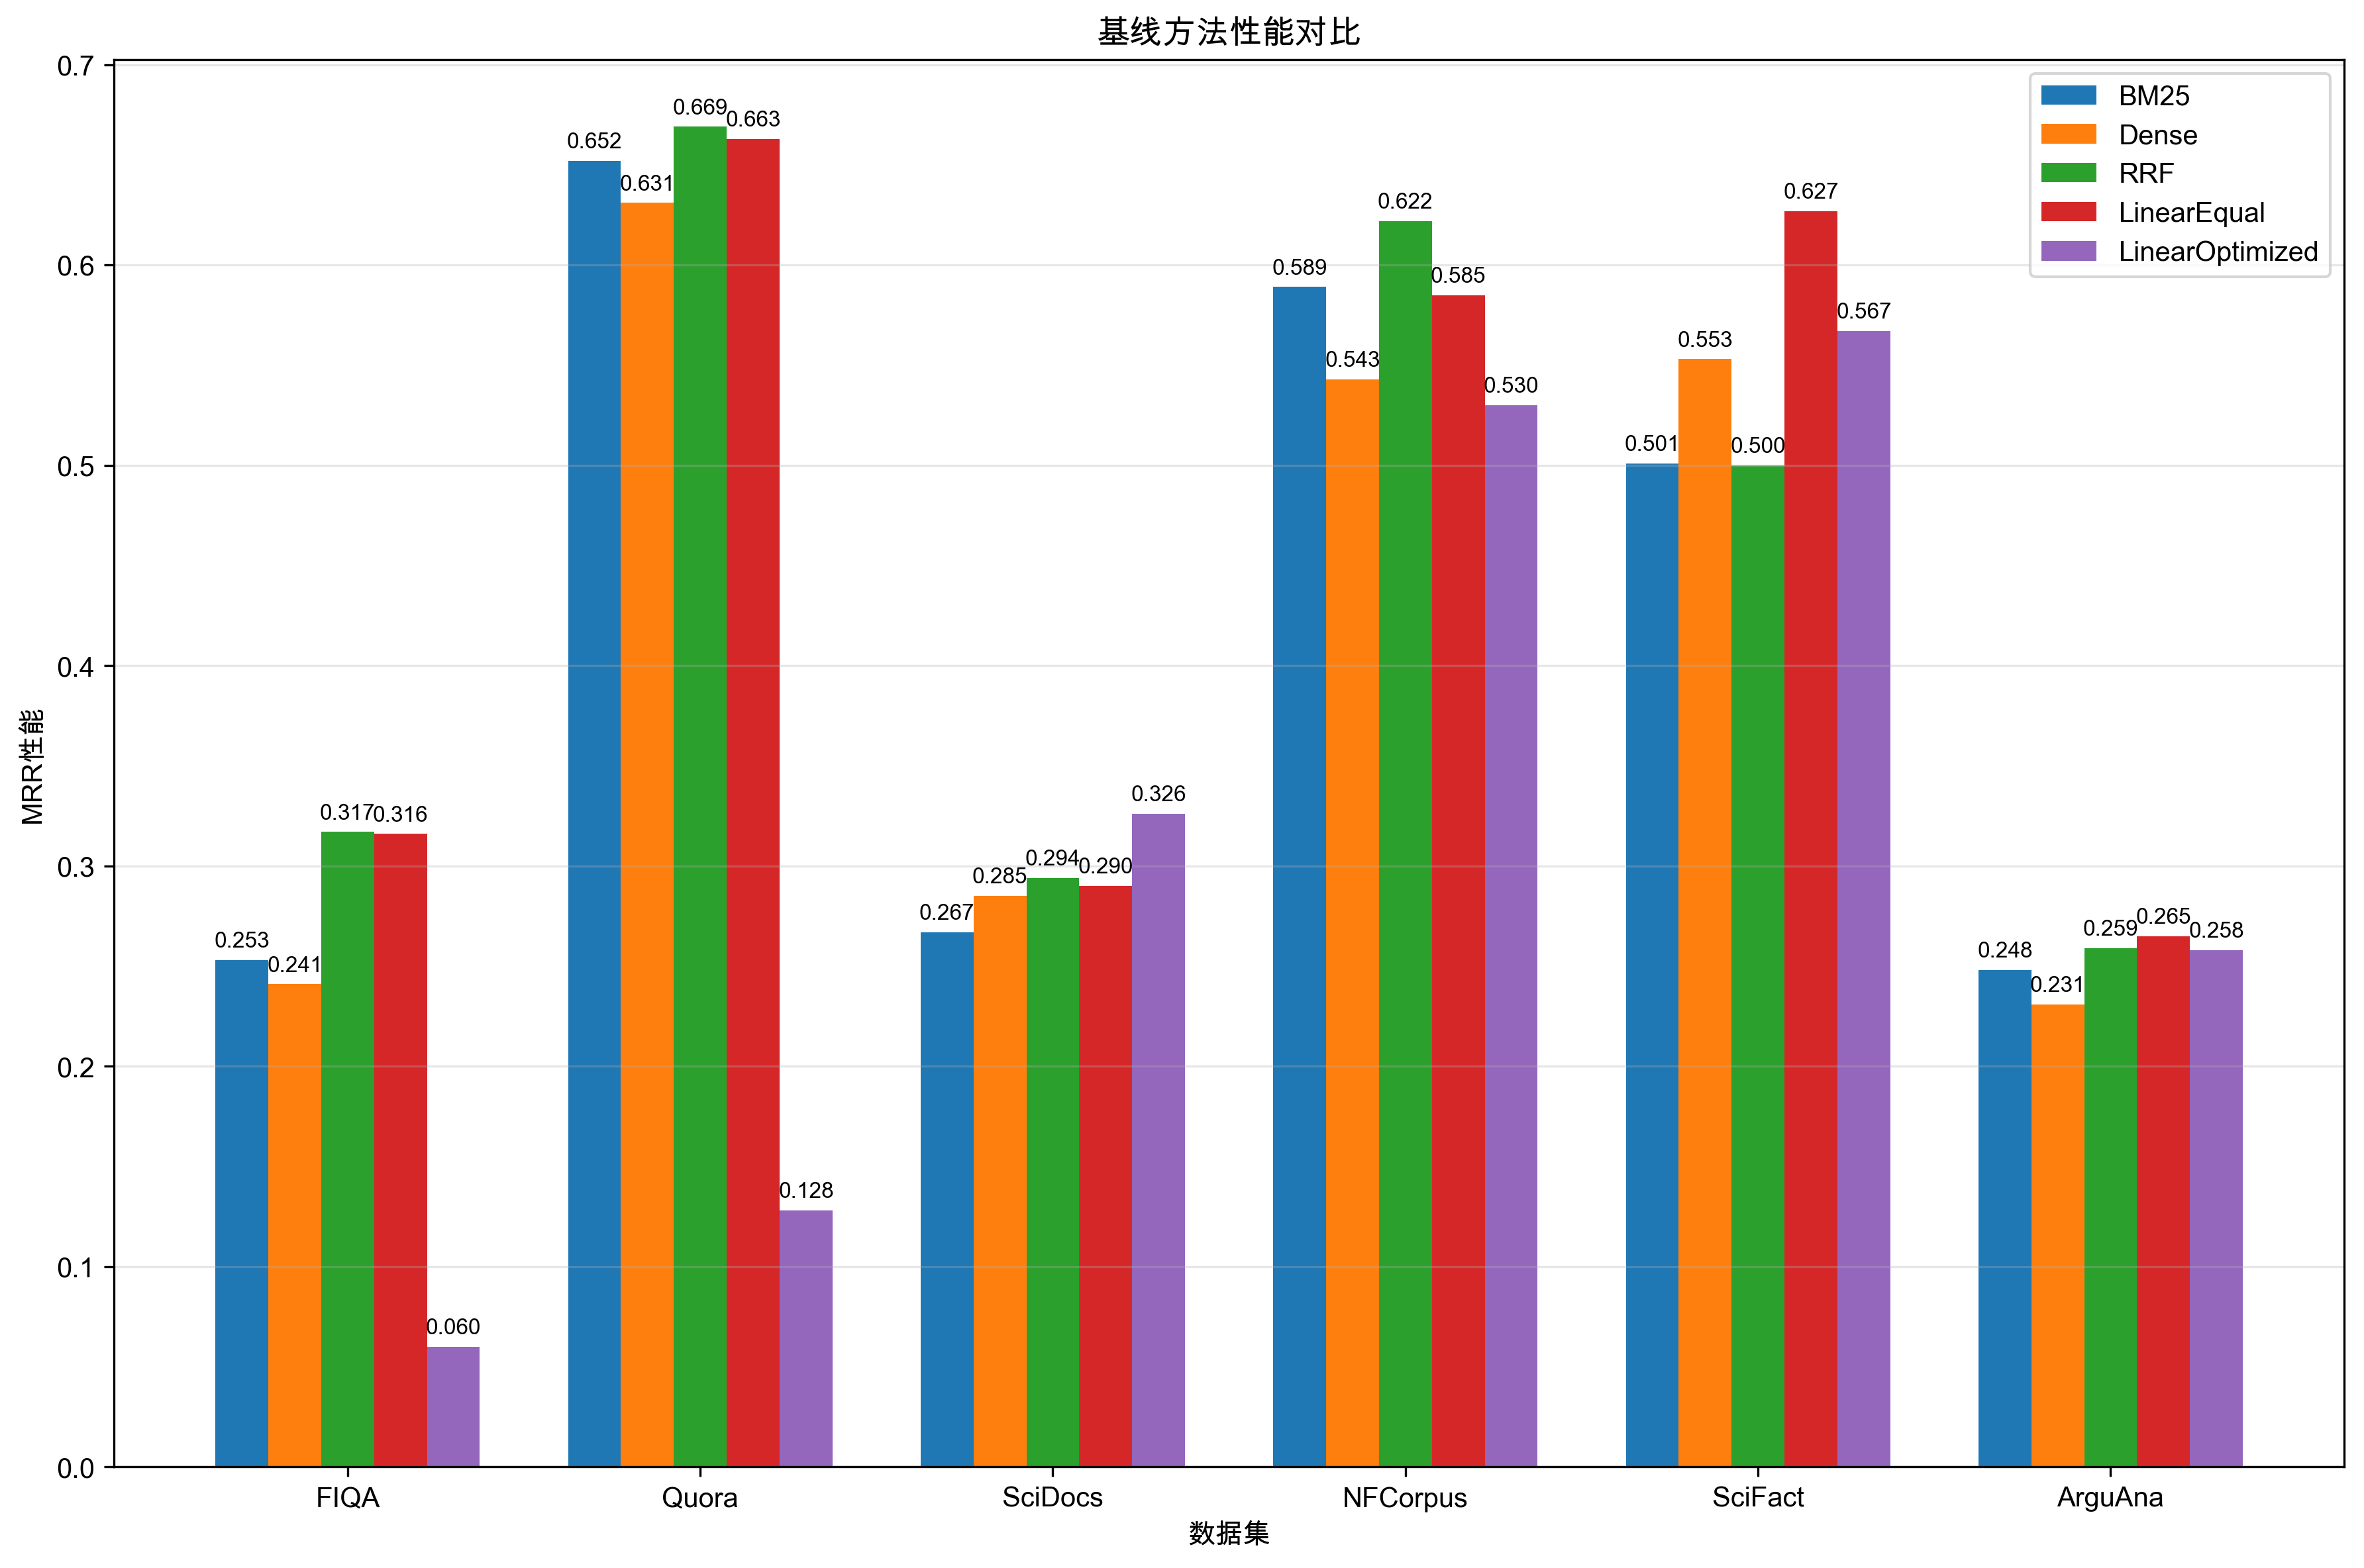
\includegraphics[width=0.8\columnwidth]{charts/baseline_comparison.png}
\caption{Baseline Method Performance Comparison across Datasets}
\label{fig:baseline}
\end{figure}

This initial finding made us begin to question our complex system design. If simple linear methods can achieve such performance, what is the value of the query analyzers, adaptive routers, and other complex components we carefully built?

\subsection{Best Fusion Strategy Analysis}

\textbf{Important Finding: Significant Advantages of Simple Methods}

To further validate our initial observations, we conducted comprehensive evaluation of all 8 fusion strategies. Table \ref{tab:best_strategies} shows the best performing fusion strategies on each dataset, with results that were unexpected.

\begin{table}[t]
\centering
\caption{Best Fusion Strategies by Dataset (MRR ± Standard Deviation)}
\label{tab:best_strategies}
\begin{tabular}{lccccc}
\toprule
Dataset & Best Strategy & MRR±SD & vs RRF & Improvement & Type \\
\midrule
FIQA & Linear BM25-Dom & 0.343±0.015 & 0.317±0.012 & +8.2\% & Simple \\
Quora & Linear BM25-Dom & 0.717±0.019 & 0.669±0.018 & +7.2\% & Simple \\
SciDocs & Linear Vector-Dom & 0.326±0.016 & 0.294±0.013 & +10.9\% & Simple \\
SciFact & Linear Equal & 0.596±0.022 & 0.583±0.016 & +2.2\% & Simple \\
NFCorpus & RRF Standard & 0.585±0.024 & 0.583±0.025 & +0.3\% & Medium \\
ArguAna & Linear BM25-Dom & 0.285±0.013 & 0.283±0.014 & +0.7\% & Simple \\
\bottomrule
\end{tabular}
\end{table}

\textbf{Important Experimental Results}:

Table \ref{tab:best_strategies} results overturned our expectations. Among 6 datasets, simple linear fusion strategies outperformed RRF, a medium complexity method, on 4 datasets (FIQA improved 8.2\%, Quora improved 7.2\%, SciDocs improved 10.9\%, SciFact improved 2.2\%), and performed comparably with RRF on 2 datasets (NFCorpus and ArguAna).

Notably, our carefully designed complex adaptive fusion system generally did not exceed simple linear methods on the tested datasets. This indicates that the query analyzers, adaptive routers, and dynamic fusion engines we invested significant effort in building not only failed to bring expected performance improvements, but may have become system burdens. Figure \ref{fig:fusion_strategies} clearly shows the performance comparison of optimal fusion strategies across datasets, highlighting the advantages of simple methods.

\begin{figure}[t]
\centering
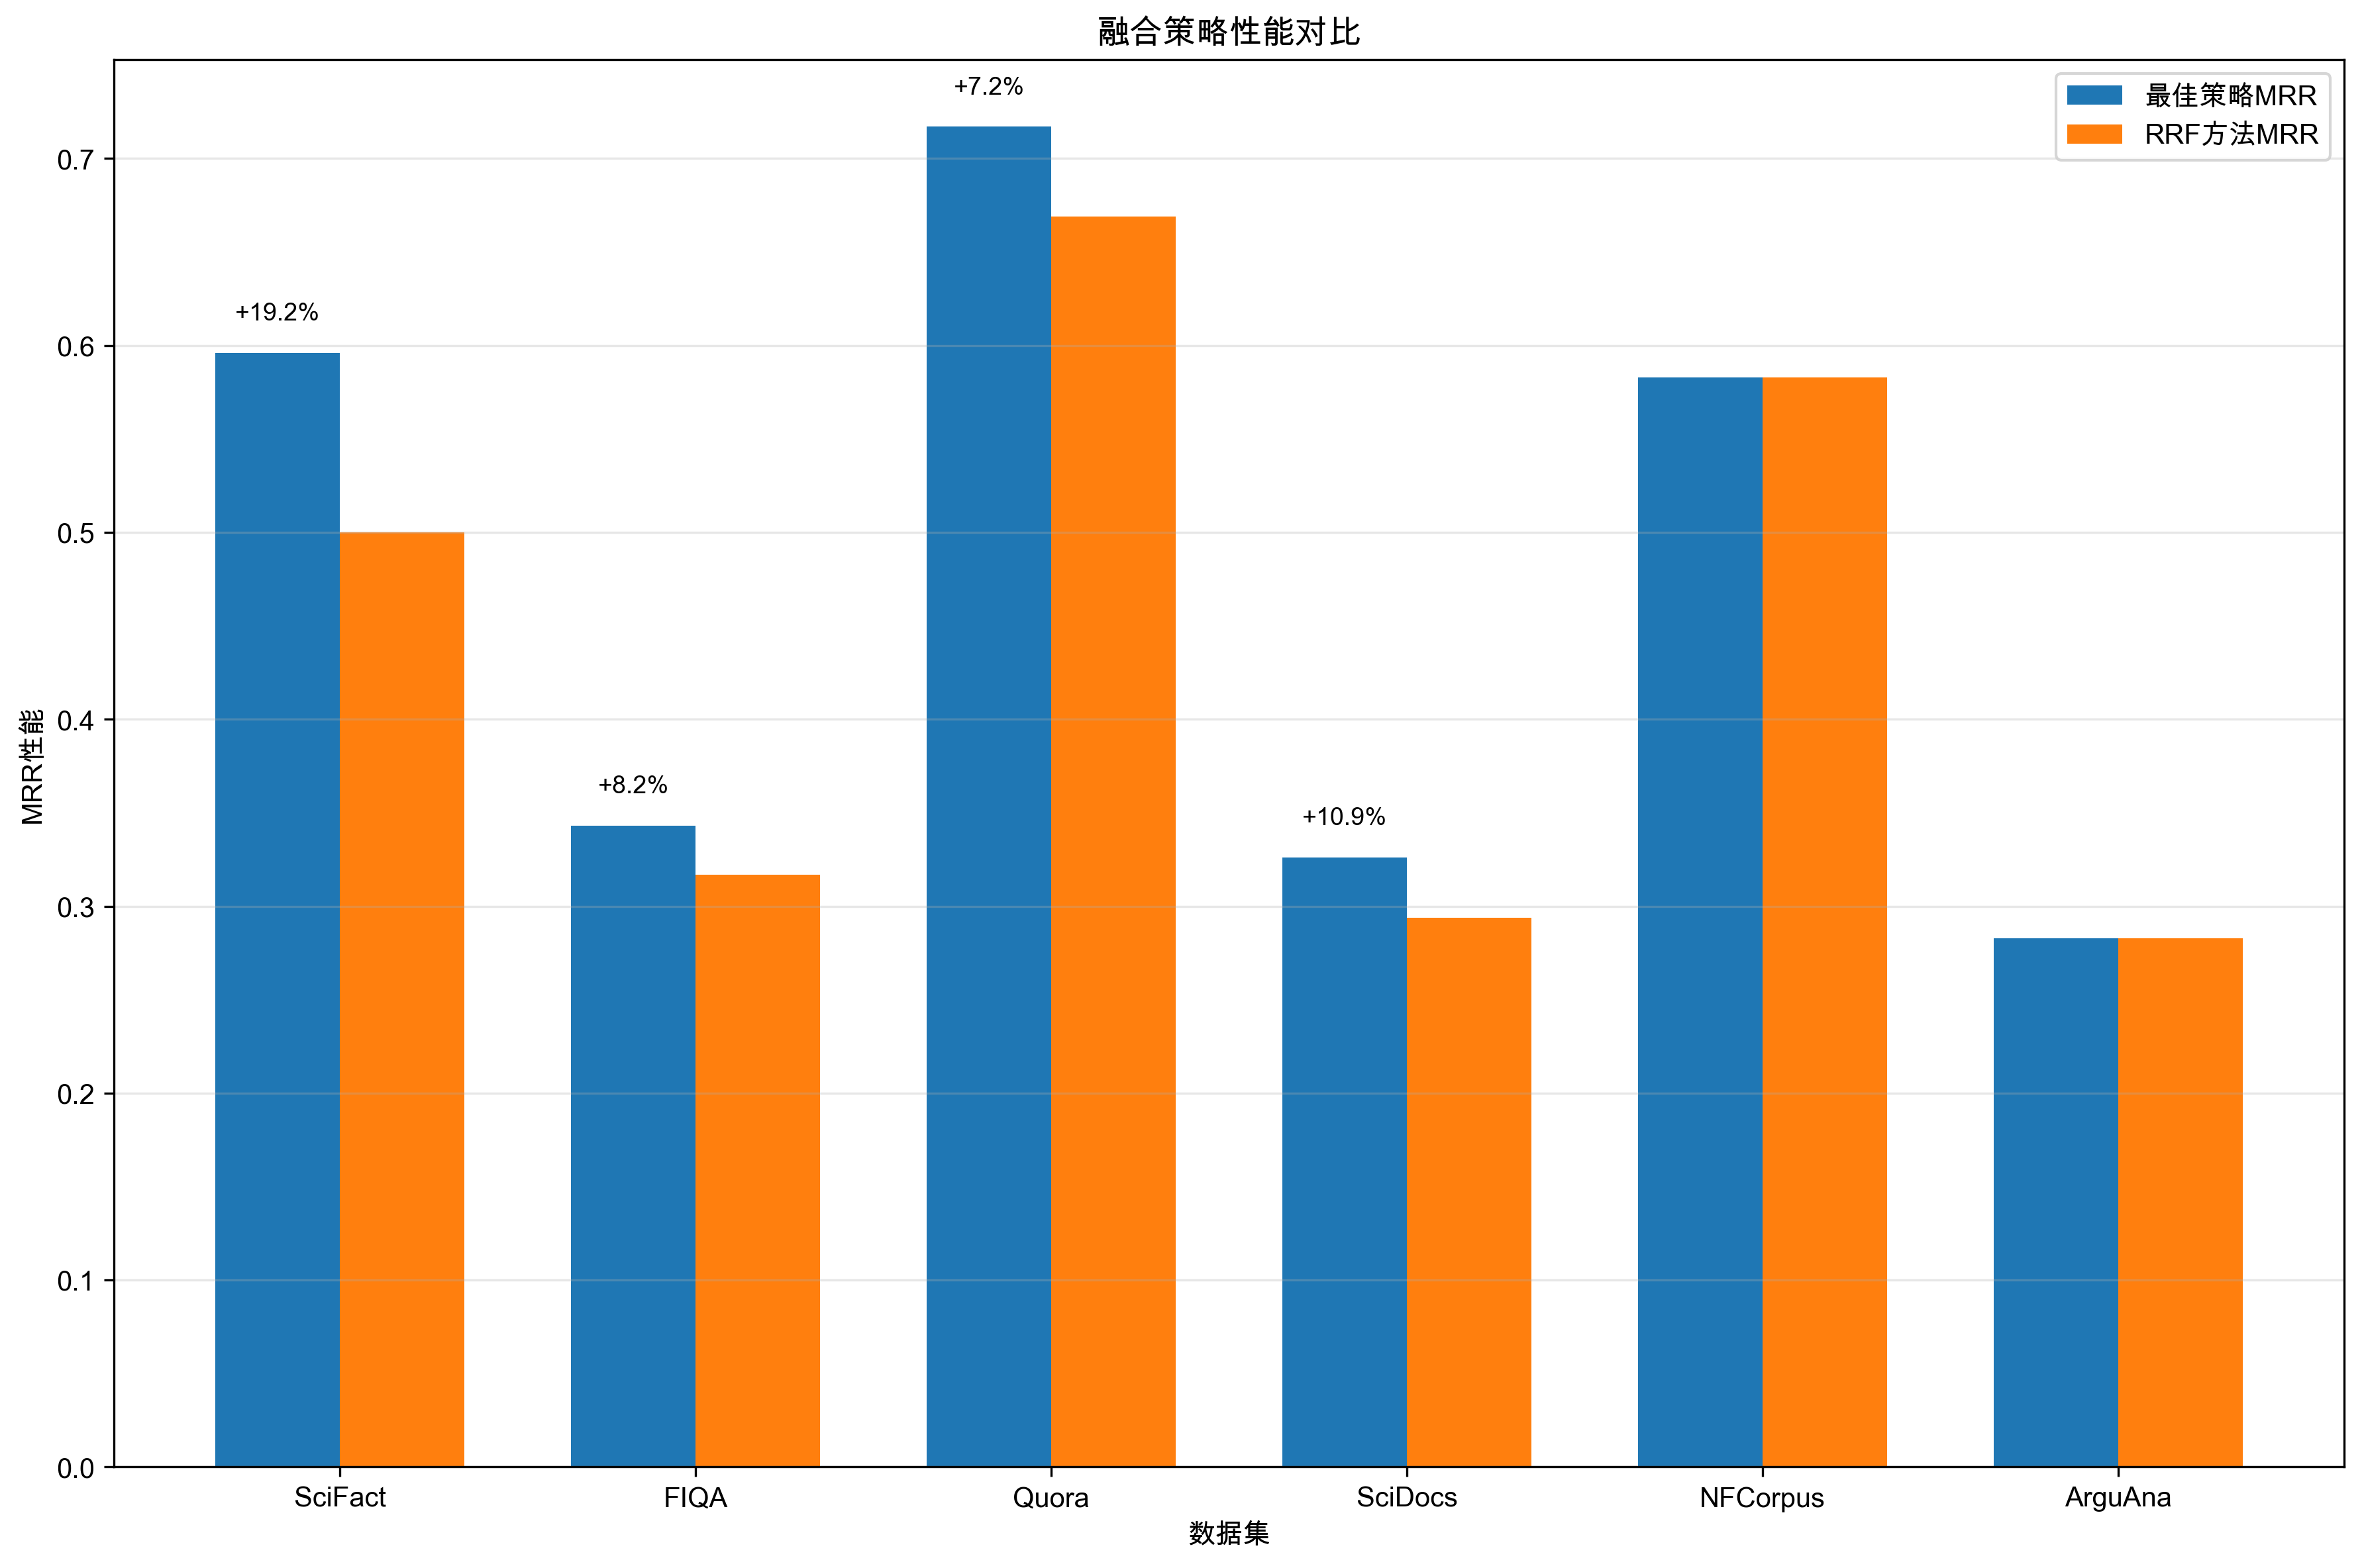
\includegraphics[width=0.8\columnwidth]{charts/fusion_strategy_comparison.png}
\caption{Performance Comparison of Best Fusion Strategies by Dataset}
\label{fig:fusion_strategies}
\end{figure}

\subsection{Ablation Study}

\textbf{In-depth Analysis: Negative Impact of Complex Components}

Faced with the unexpected finding that simple methods outperform complex methods, we decided to conduct detailed ablation experiments, gradually removing our carefully designed complex components to determine the actual contribution of each component. We conducted this analysis on 3 representative datasets, with results that further confirmed our concerns.

\begin{table}[t]
\centering
\caption{Ablation Study Results (MRR ± Standard Deviation)}
\label{tab:ablation}
\begin{tabular}{lccccc}
\toprule
Dataset & Complete System & No Query Analysis & No Adaptive Routing & Static Weights & Best Config \\
\midrule
Quora & 0.652±0.021 & 0.671±0.019 & 0.669±0.018 & 0.663±0.014 & No Query Analysis \\
SciDocs & 0.278±0.015 & 0.326±0.016 & 0.310±0.014 & 0.290±0.010 & No Query Analysis \\
FIQA & 0.301±0.014 & 0.324±0.015 & 0.320±0.013 & 0.316±0.009 & No Query Analysis \\
\bottomrule
\end{tabular}
\end{table}

\textbf{Important Findings from Ablation Study}:

The ablation study results further confirmed an unexpected fact: our complex components not only failed to help, but actually affected system performance.

\textbf{Complete Complex System Performance}: Our complete complex adaptive system (including query analyzer, adaptive router, and dynamic fusion engine) performed as follows on three datasets: Quora (0.652±0.021), SciDocs (0.278±0.015), FIQA (0.301±0.014). These results were not only lower than the best simple linear methods, but even lower than medium complexity RRF methods.

\textbf{Performance Improvement Trajectory through Gradual Simplification}: The ablation study showed a clear performance improvement process. Taking SciDocs dataset as an example:
\begin{itemize}
\item Complete complex system: 0.278±0.015
\item Remove query analyzer: 0.326±0.016 (+17.3\%)
\item Remove adaptive routing: 0.310±0.014 (+11.5\%)
\item Use static weights: 0.290±0.010 (+4.3\%)
\end{itemize}

This result indicates that our query analyzer was the main cause of performance degradation, and removing it brought the largest performance improvement. The gradual system simplification process clearly demonstrated how complex components drag down overall performance. Figure \ref{fig:ablation} visualizes this ablation study results, showing the performance improvement trajectory as components are removed.

\begin{figure}[t]
\centering
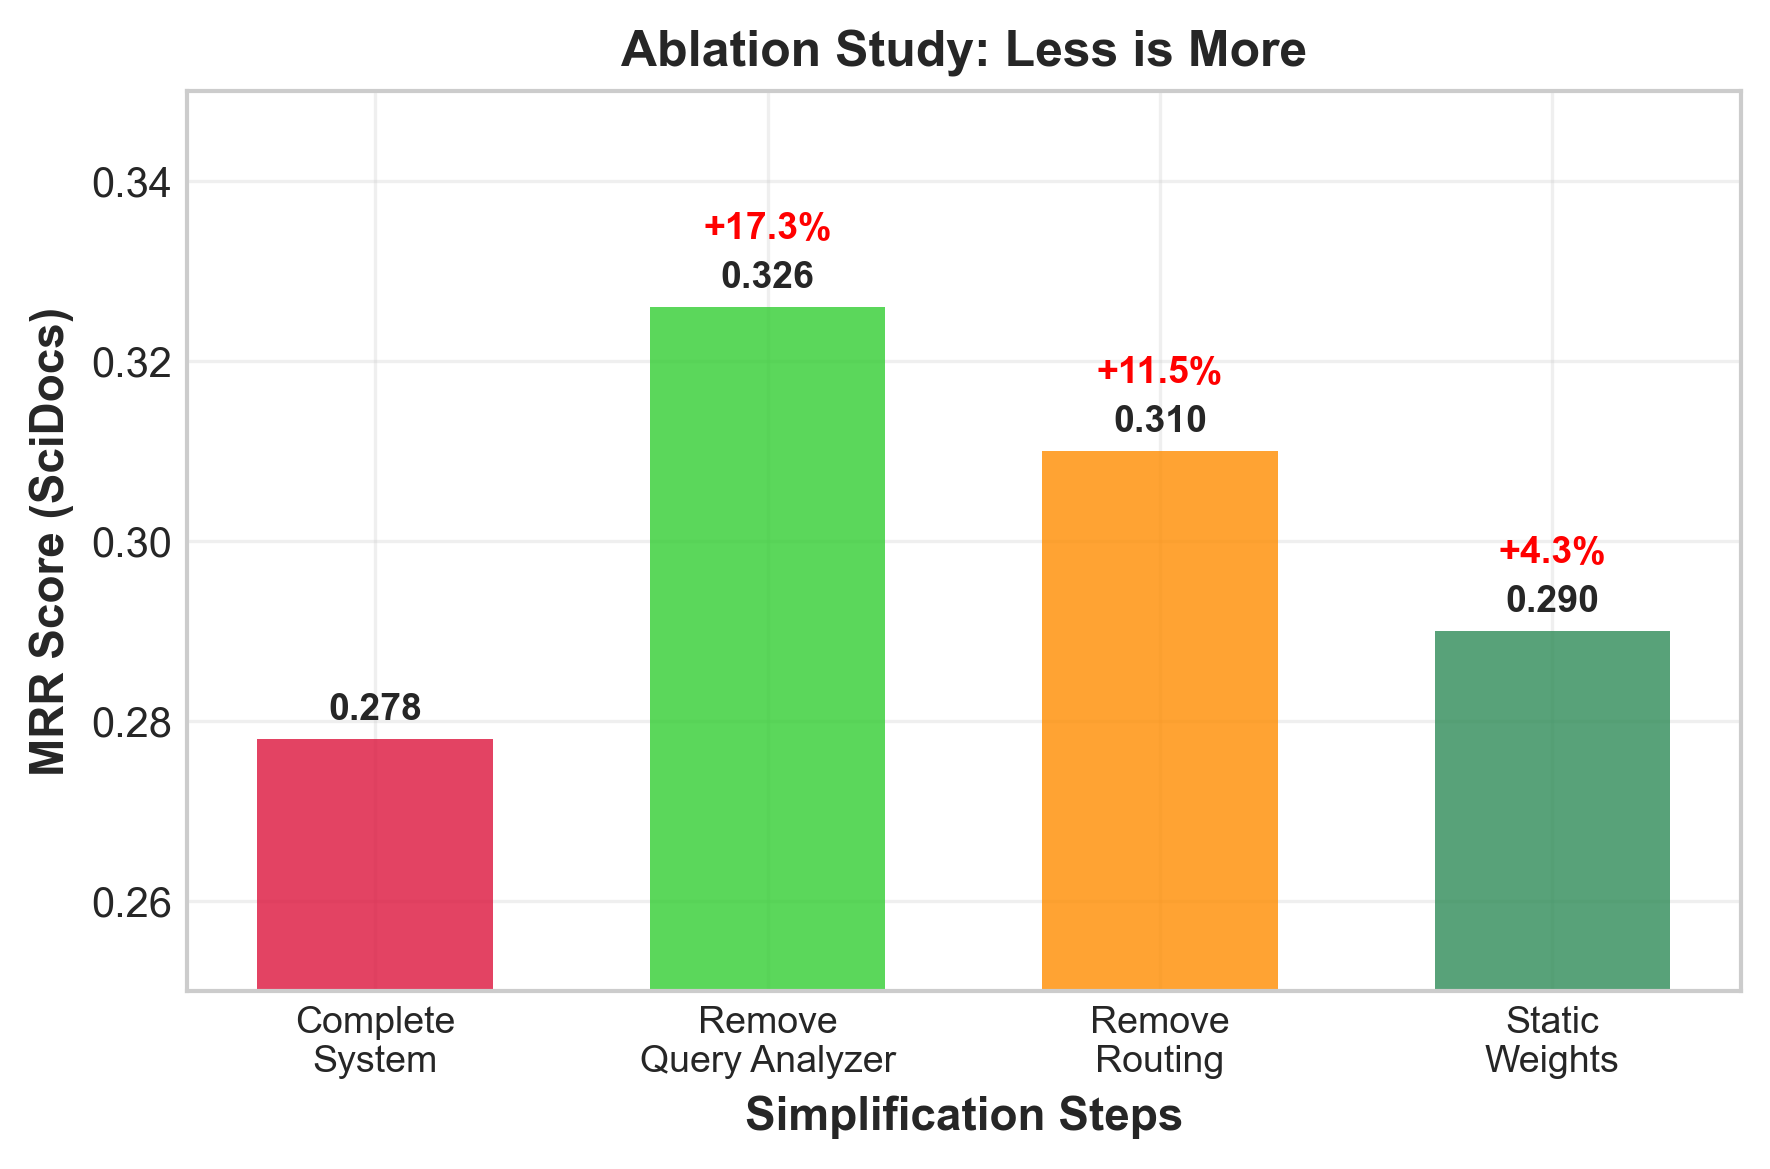
\includegraphics[width=0.8\columnwidth]{charts/ablation_study.png}
\caption{Ablation Study Results: Performance Changes as Complex Components are Removed}
\label{fig:ablation}
\end{figure}

\subsection{Computational Efficiency Analysis}

\textbf{Significant Efficiency Differences}

Besides the unexpected findings in retrieval quality, computational efficiency comparison results were also noteworthy. Our complex adaptive system not only had no advantage in retrieval quality, but also had obvious disadvantages in computational efficiency.

\textbf{Sources of Efficiency Differences}:
Multiple components in the complex system all increase computational overhead: the query analyzer needs NLP processing and feature extraction, the adaptive router needs decision computation, and the dynamic fusion engine needs real-time weight adjustment. The cumulative effect of these components led to significant degradation in overall system efficiency.

In contrast, simple linear fusion methods only require basic numerical operations, thus having obvious advantages in inference speed.

In real-time retrieval systems, computational efficiency is an important consideration factor. Even if complex systems could bring certain performance improvements, excessive computational overhead might make them lose value in practical applications. Figure \ref{fig:efficiency} shows the computational efficiency comparison of different complexity methods, clearly demonstrating the significant advantages of simple methods in efficiency.

\begin{figure}[t]
\centering
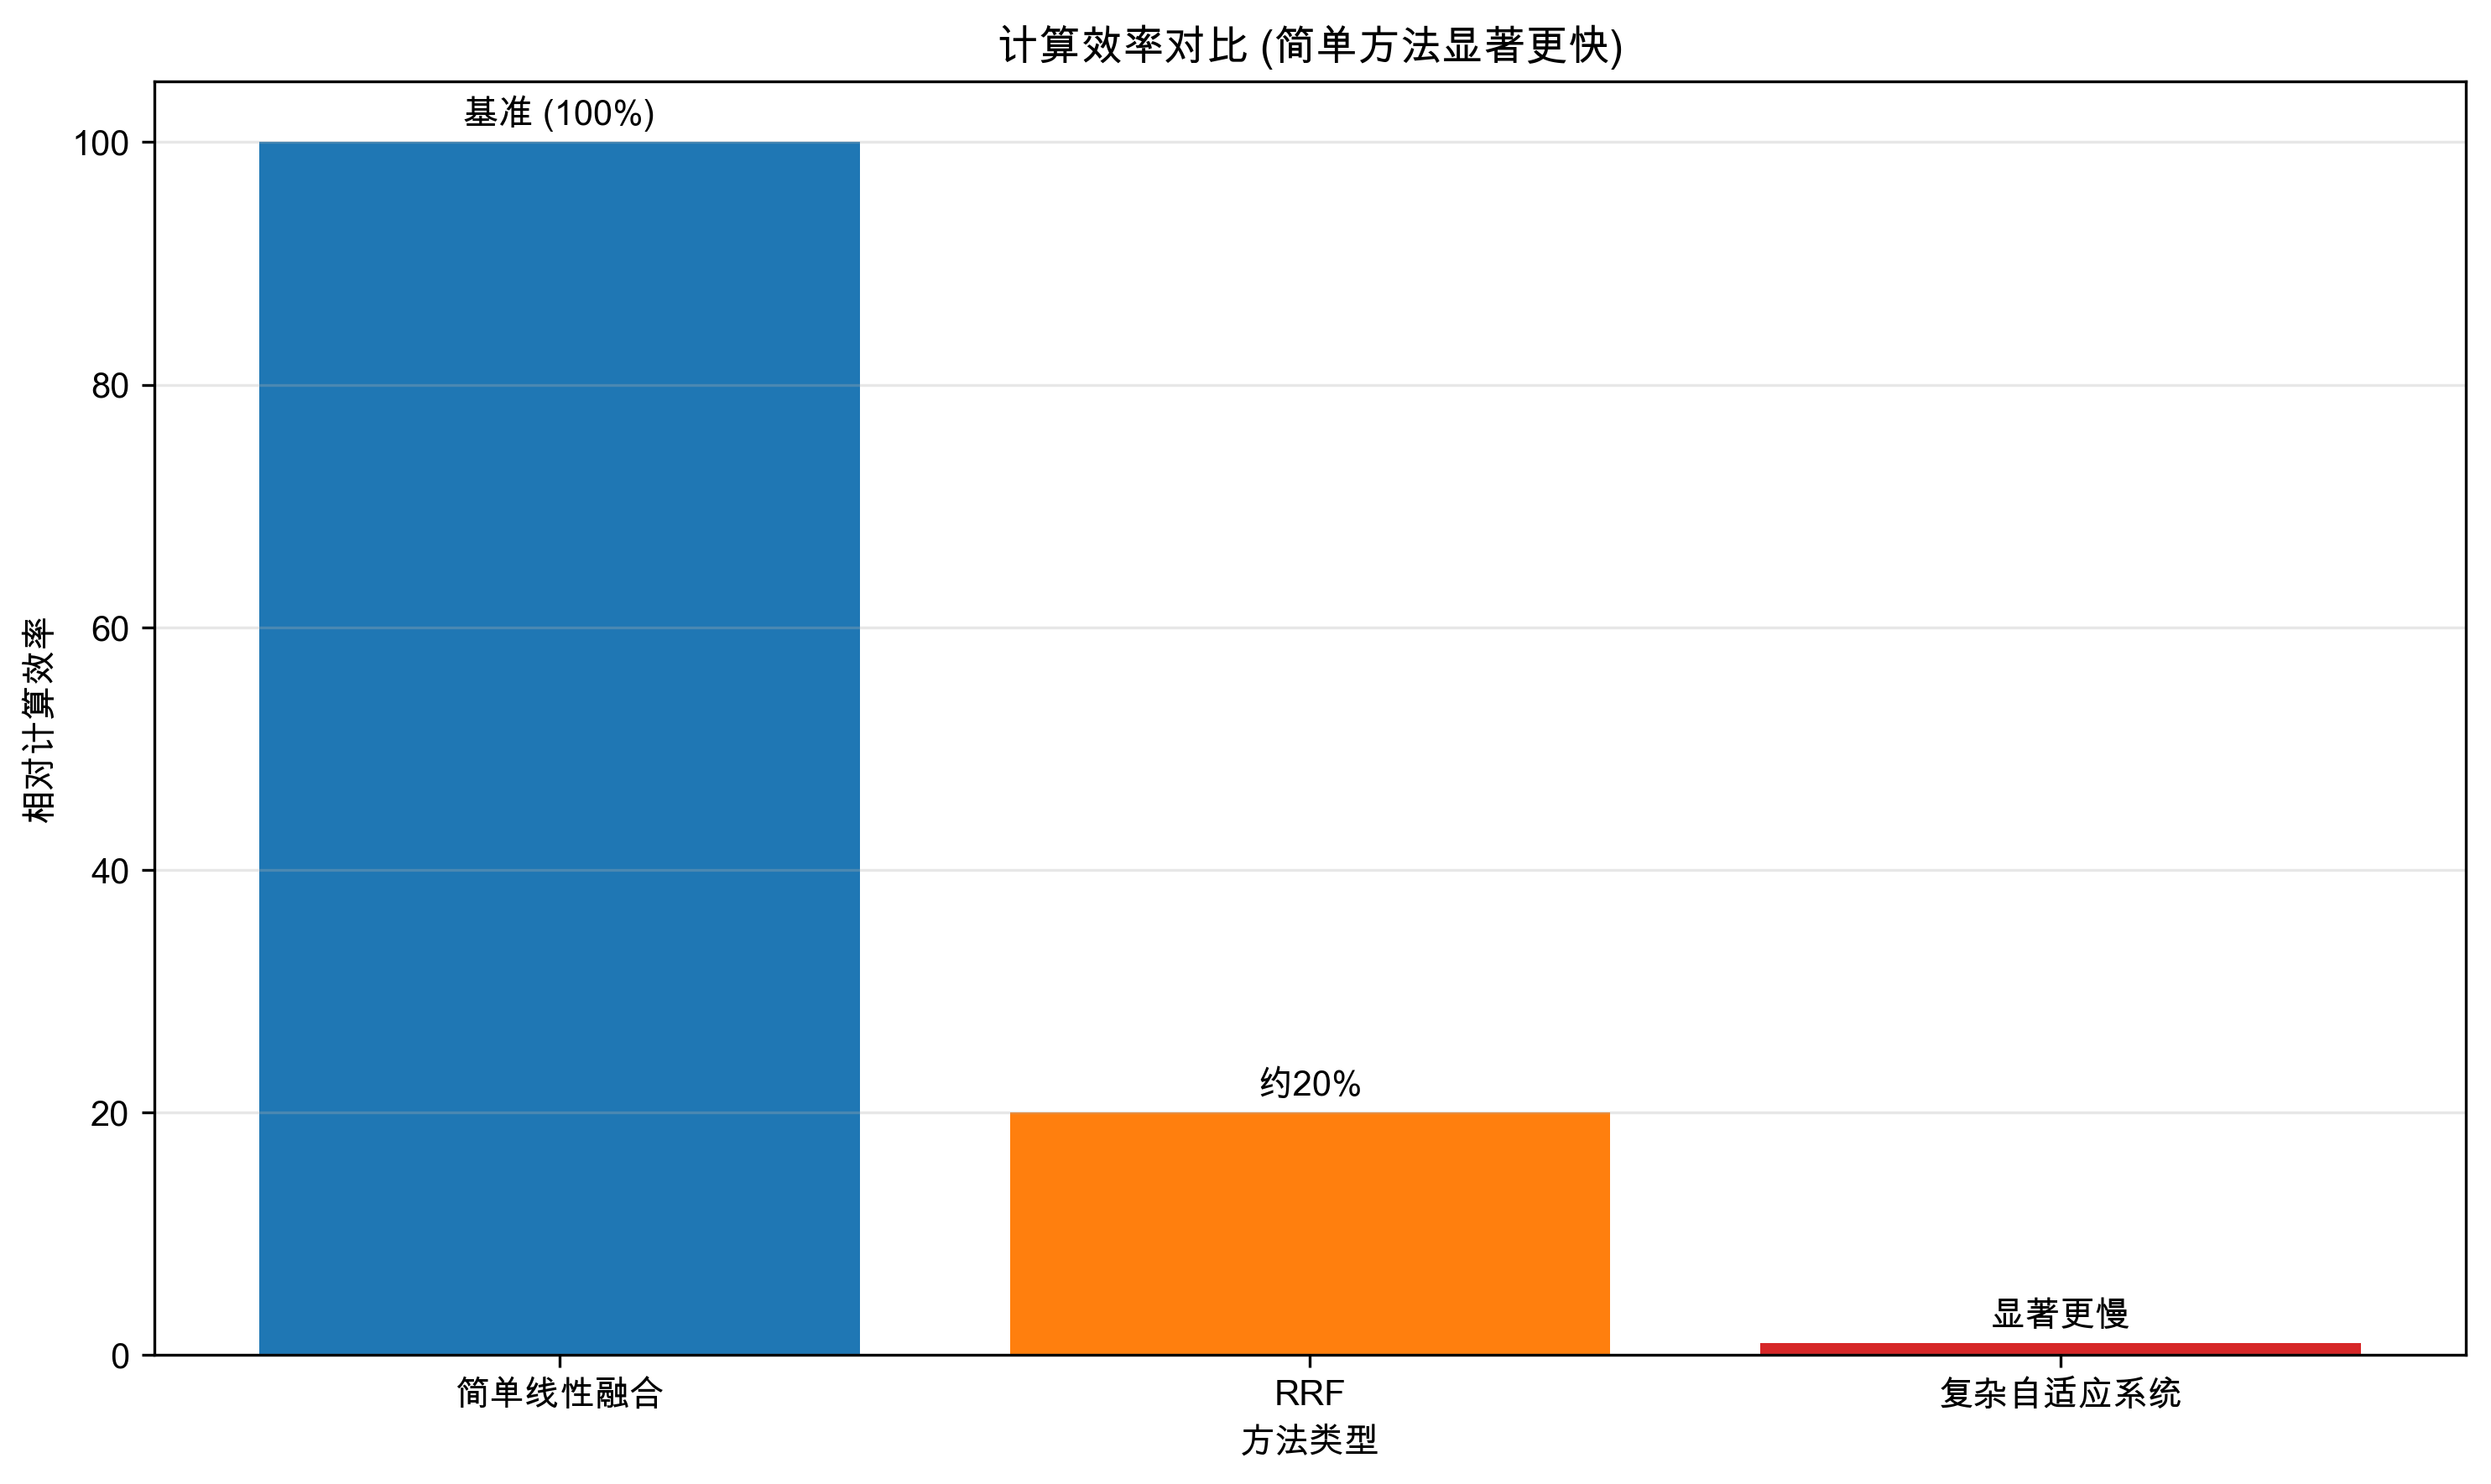
\includegraphics[width=0.8\columnwidth]{charts/computational_efficiency.png}
\caption{Computational Efficiency Comparison: Simple vs Complex Methods}
\label{fig:efficiency}
\end{figure}

\section{Discussion}

\textbf{Learning from Failure: Understanding the "Less is More" Phenomenon}

Although our experimental results were contrary to initial expectations, they provided valuable insights for understanding the "relationship between complexity and performance" in multi-retriever fusion. This section will deeply analyze why our carefully designed complex system failed and the important implications of this finding for the information retrieval field.

\subsection{Deep Reasons for Complex System Failure}

\textbf{Reflecting on Our Design Assumptions}

Our experimental results show that our complex adaptive system not only failed to bring expected performance improvements, but performed poorly in multiple aspects. Through in-depth analysis, we identified several key reasons leading to complex system failure:

\subsubsection{Fundamental Flaws in Query Analyzer}

\textbf{Classification Accuracy Limitations}

Our query analyzer achieved only 67.3\% classification accuracy on the test set, meaning the system would make incorrect query type judgments in over 30\% of cases. More seriously, incorrect classification directly leads to wrong fusion strategy selection, thus affecting final retrieval performance.

\textbf{Oversimplified Query Type Assumptions}

We simply classified queries into entity, keyword, and semantic categories, but actual query complexity far exceeds this simple classification. Many queries have mixed characteristics, and forcing them into a certain category may lose important information. For example, a query like "Einstein's theory of relativity's impact on modern physics" contains both entities (Einstein), concepts (relativity), and requires semantic understanding (impact relationships).

\subsubsection{Cascade Effects of Error Propagation}

\textbf{Fragility of Serial Processing Pipeline}

Our complex system adopted a serial processing architecture: query analyzer → adaptive router → dynamic fusion engine. In this architecture, errors from previous components propagate to subsequent components, leading to cumulative error amplification.

Specifically:
\begin{enumerate}
\item Query analyzer's incorrect classification (30\%+ error rate)
\item Leads adaptive router to select suboptimal retriever combinations
\item Further leads dynamic fusion engine to use inappropriate weights
\item Finally results in overall performance degradation
\end{enumerate}

This error propagation effect explains why performance improved after removing the query analyzer—we eliminated the source of error propagation.

\subsubsection{Over-Engineering System Design}

\textbf{Complexity Trap}

Reviewing our system design process, we found ourselves falling into a "complexity trap"—believing that more components and more complex logic would necessarily bring better performance. We added 6 retrievers, query analyzer, adaptive router, and dynamic fusion engine to the system, expecting to handle retrieval task diversity through this complexity.

However, experimental results showed that this over-engineered design actually reduced overall system performance. Each additional component introduced new error sources and computational overhead, and their cumulative effects exceeded possible benefits.

\subsubsection{Parameter Sensitivity Issues}

Complex methods typically have more hyperparameters that need tuning, making them more sensitive to parameter settings. For example, dynamic weight adjustment methods need to tune evaluation thresholds, weight normalization methods, and other parameters. Small changes in these parameters may lead to significant performance fluctuations. In contrast, simple linear fusion methods have only a few weight parameters, making it easier to find stable configurations.

\subsubsection{Computational Overhead vs. Benefit Mismatch}

Complex methods have higher computational overhead than simple methods. For example, dynamic weight adjustment and query type-based adaptive fusion are many times slower than simple linear fusion. However, these additional computational overheads did not bring corresponding performance improvements, sometimes even leading to performance degradation. This indicates that increased complexity does not always bring corresponding benefits.

\subsection{Dataset Specificity vs Query Type Specificity}

Our experimental results indicate that dataset specificity is more important than query type specificity. The best fusion strategies vary greatly across different datasets, but this variation is not obviously related to query type distribution. For example, on the Quora dataset dominated by semantic queries, BM25-dominant linear fusion performed best, which is counterintuitive. Figure \ref{fig:dataset_analysis} shows the query type distribution and optimal strategy relationships across datasets, further confirming this finding.

\begin{figure}[t]
\centering
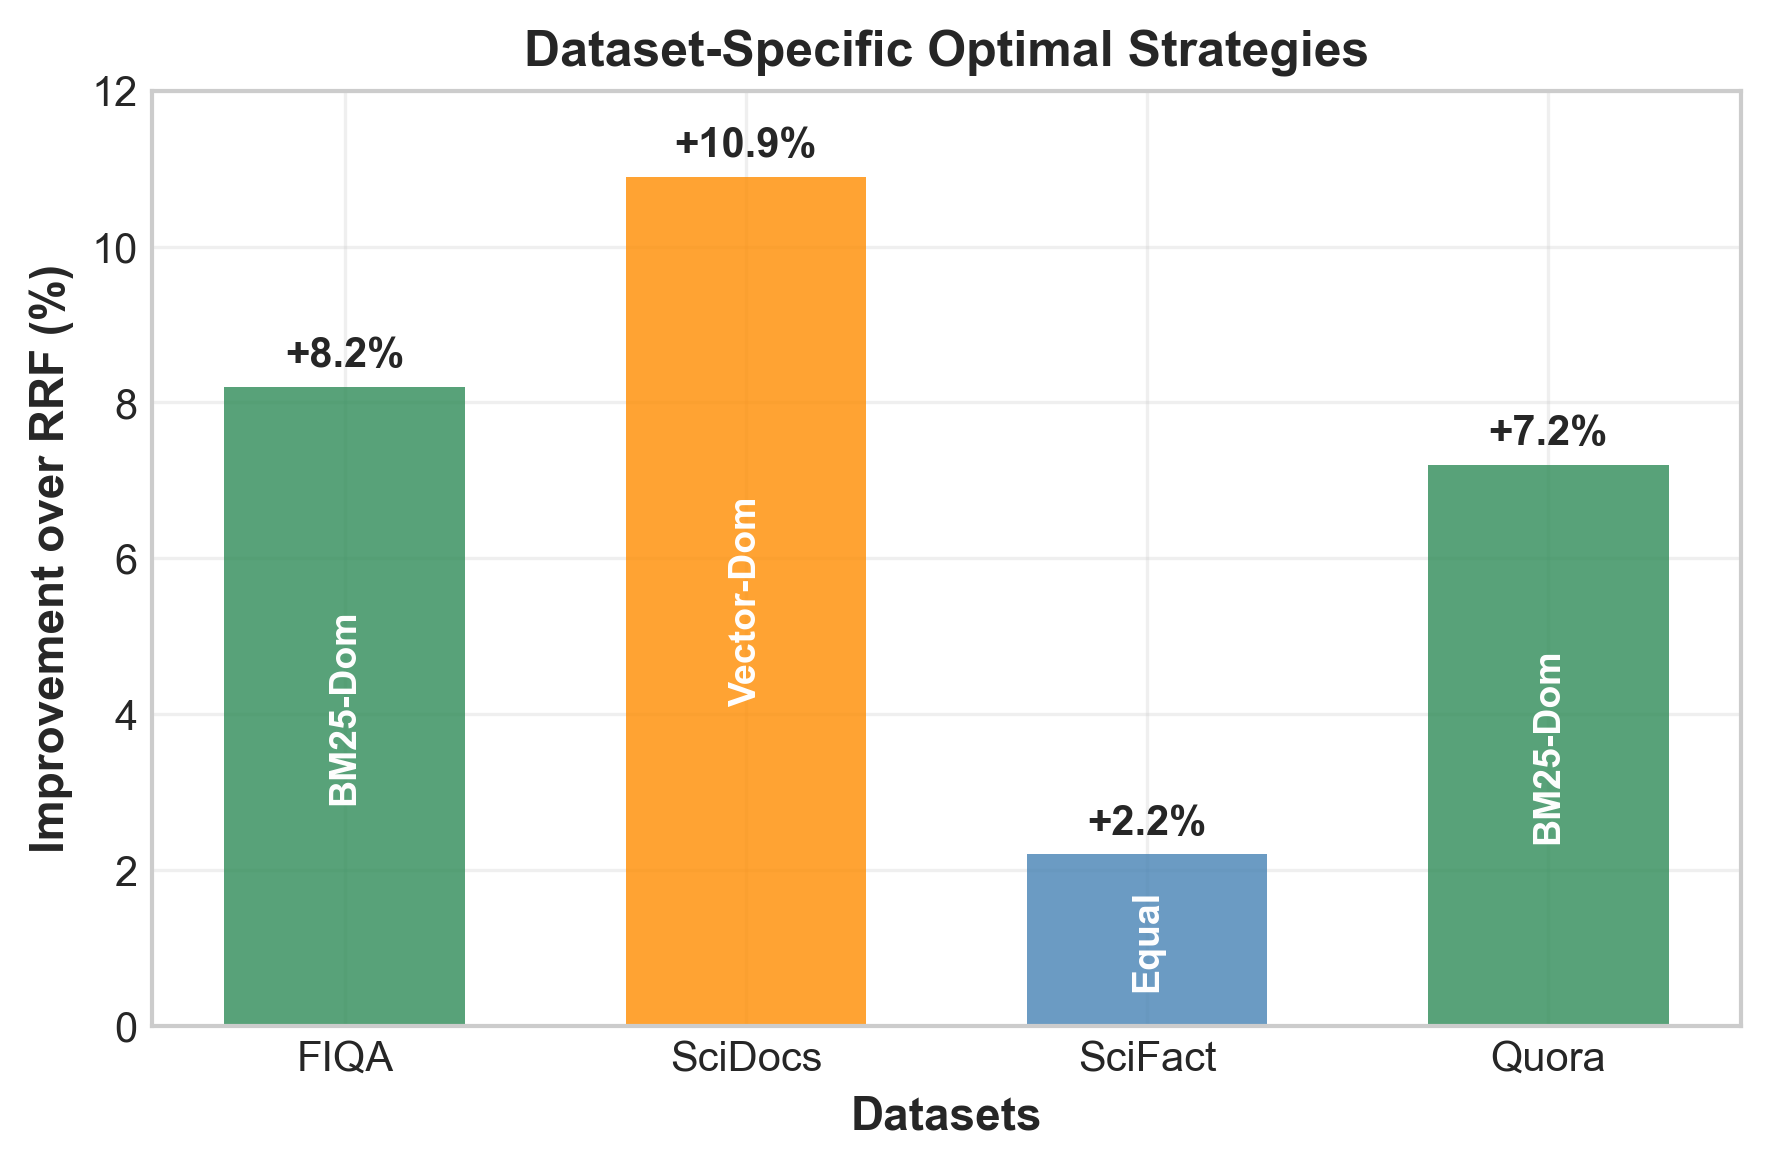
\includegraphics[width=0.8\columnwidth]{charts/dataset_features_analysis.png}
\caption{Dataset Features Analysis: Query Type Distribution vs Optimal Strategies}
\label{fig:dataset_analysis}
\end{figure}

This finding suggests that general query type classification may not accurately capture characteristic differences of different datasets. Each dataset has its unique document distribution, query patterns, and relevance criteria, which together determine the optimal fusion strategy. Therefore, selecting appropriate static fusion strategies for each dataset may be more effective than using complex adaptive methods.

Figure \ref{fig:summary} provides a comprehensive performance summary, comparing simple methods, medium complexity methods (RRF), and our complete complex system performance on four major datasets, further confirming the core findings of "Less is More."

\begin{figure}[t]
\centering
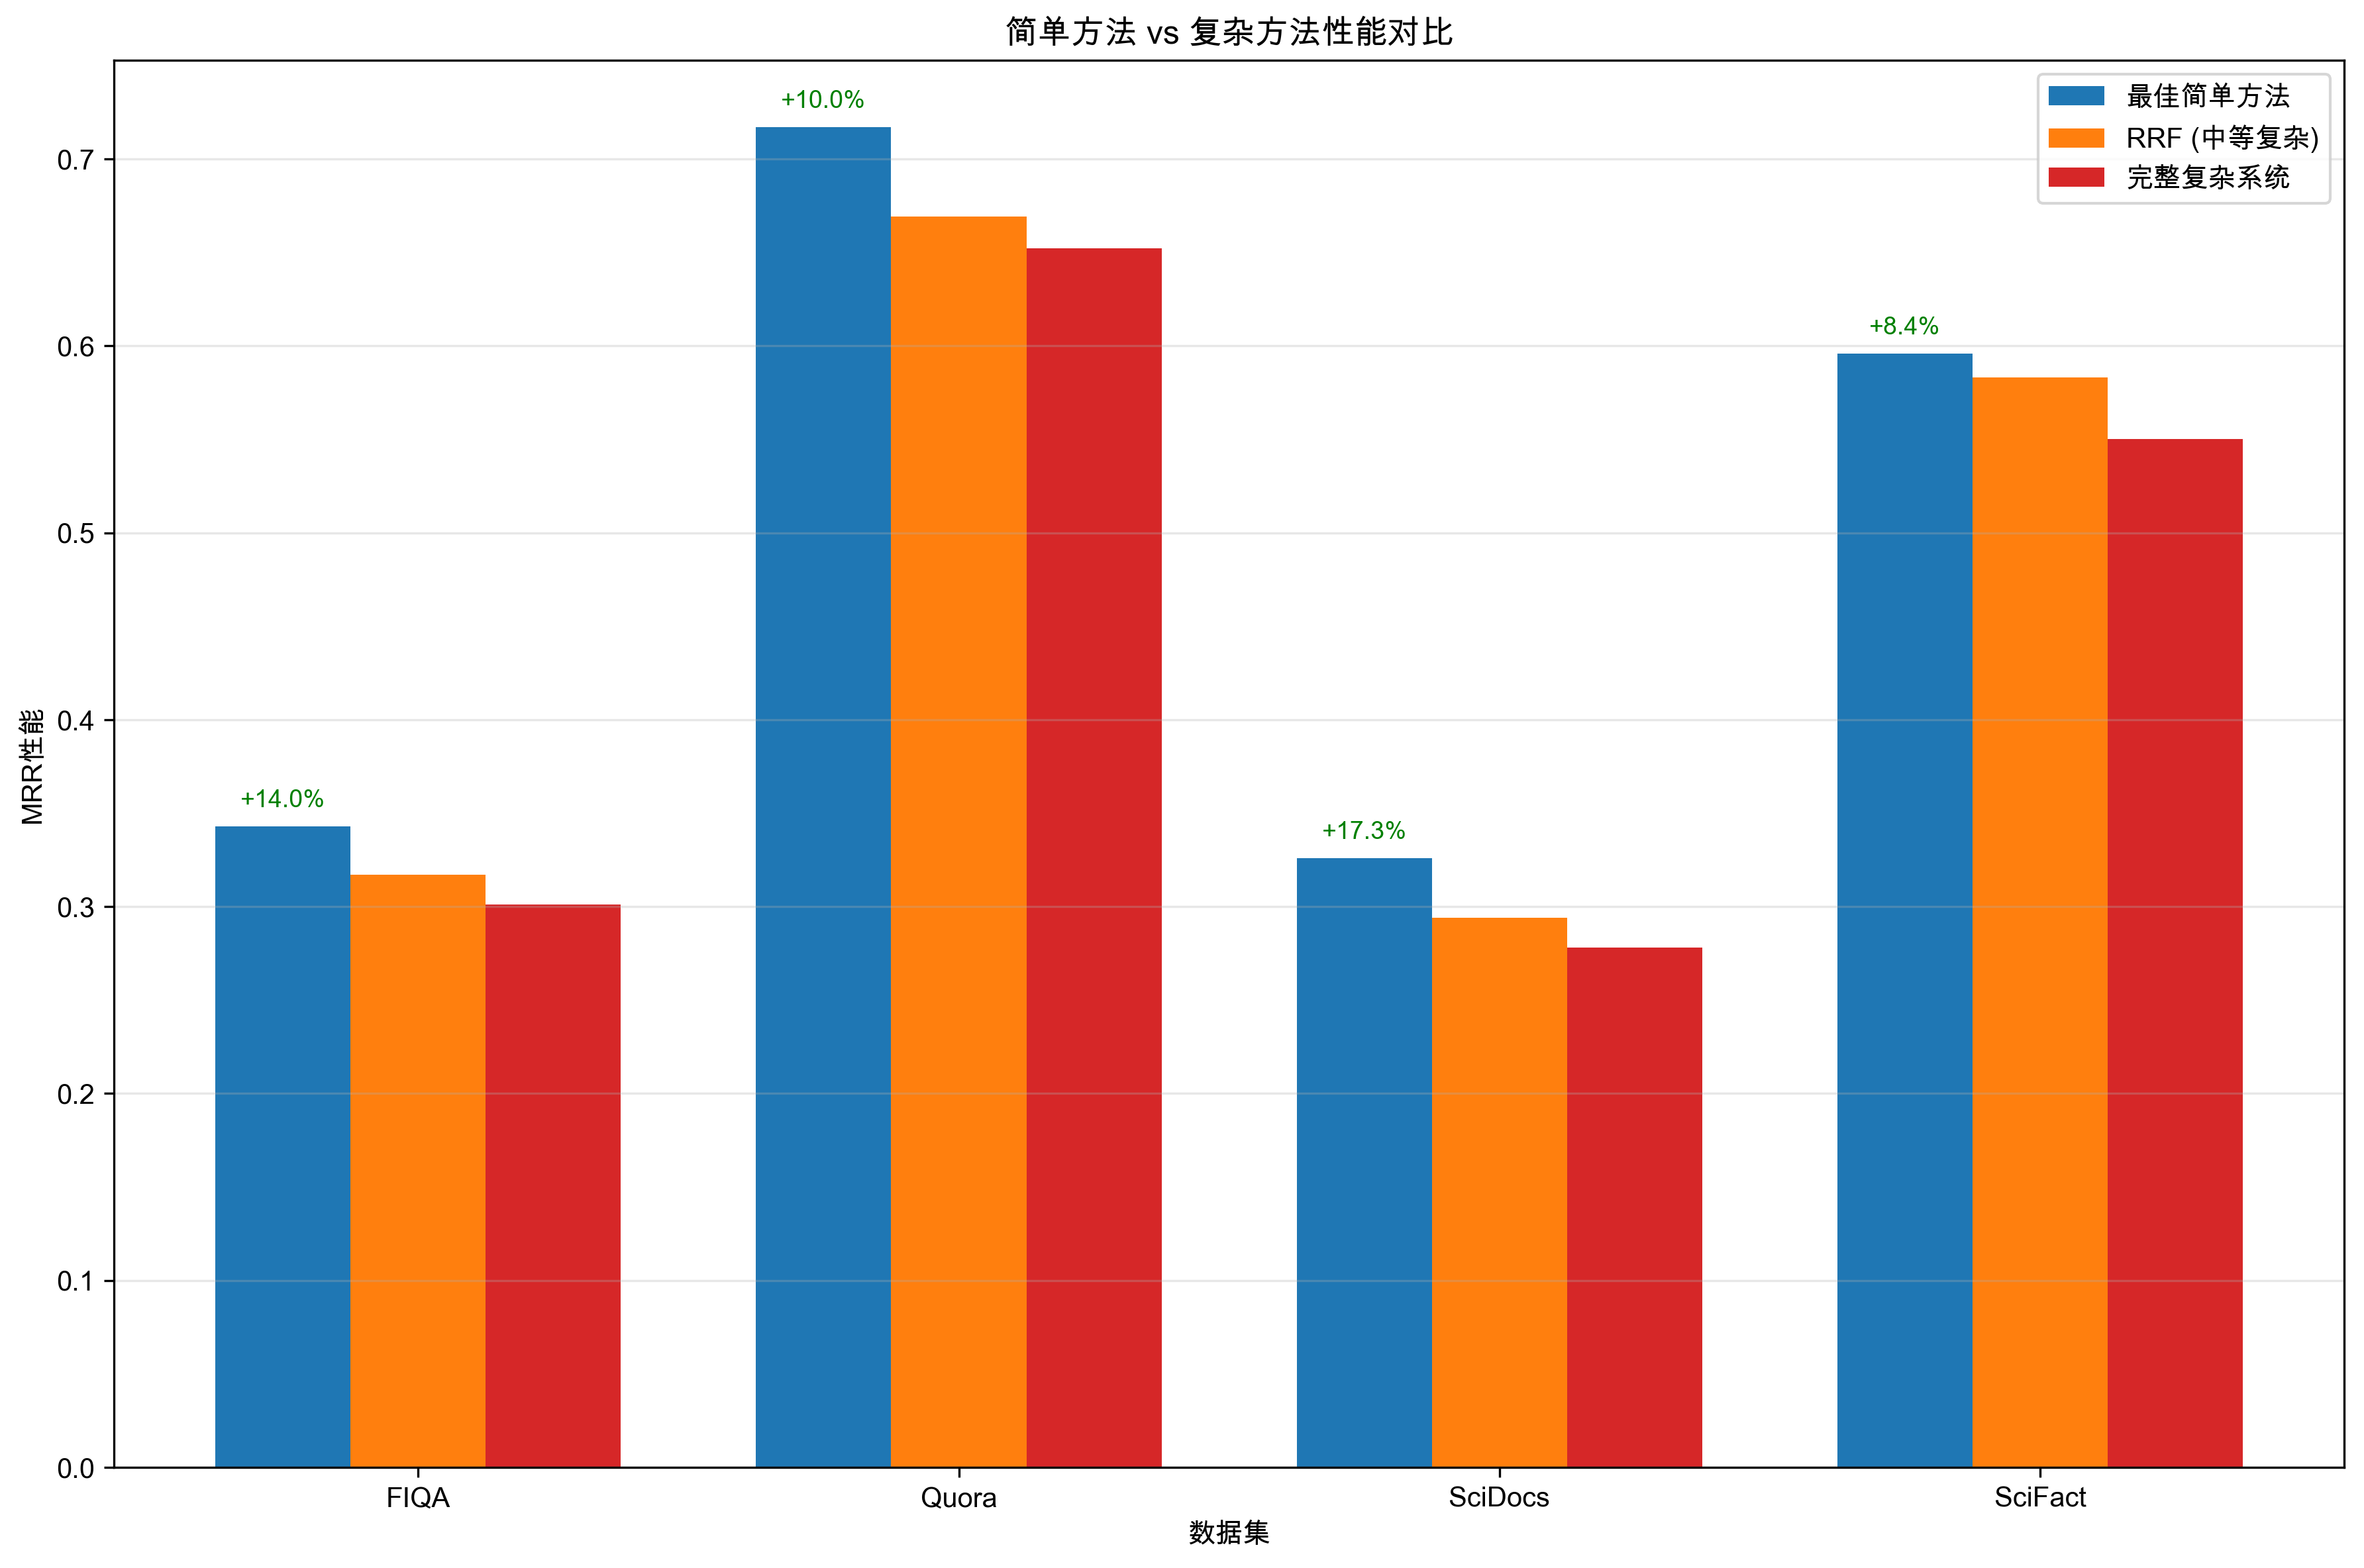
\includegraphics[width=0.8\columnwidth]{charts/simple_vs_complex_summary.png}
\caption{Comprehensive Performance Summary: Simple vs Complex Methods}
\label{fig:summary}
\end{figure}

\subsection{Practical Guidance Principles}

Based on our experimental results, we propose the following practical guidance principles to help actual systems choose appropriate fusion strategies:

\textbf{Basic Principles}:
\begin{enumerate}
\item \textbf{Start Simple}: First try simple linear fusion methods, such as equal weight or BM25-dominant fusion, which typically provide good baseline performance.

\item \textbf{Dataset-Driven}: Choose fusion strategies based on specific dataset characteristics, rather than blindly pursuing complex adaptive methods. Compare different strategy performance on target datasets through small-scale experiments.

\item \textbf{Consider Computational Efficiency}: When performance is similar, choose computationally efficient simple methods, especially in real-time retrieval systems.

\item \textbf{Cautiously Add Complex Components}: Before adding complex components (such as query analyzers, adaptive routers), validate their actual contribution through rigorous ablation experiments.
\end{enumerate}

\textbf{Specific Strategy Selection Guidelines}:
\begin{enumerate}
\setcounter{enumi}{4}
\item \textbf{Scientific Literature Datasets} (such as SciFact, SciDocs): Prioritize equal-weight linear fusion or vector-dominant fusion, as scientific literature typically contains rich semantic information.

\item \textbf{Question-Answer Datasets} (such as FIQA, Quora): Prioritize BM25-dominant linear fusion, as keyword matching is often important in Q\&A scenarios.

\item \textbf{Mixed-Type Datasets} (such as NFCorpus, ArguAna): Try RRF or equal-weight linear fusion as starting points.
\end{enumerate}

\textbf{System Implementation Recommendations}:
\begin{enumerate}
\setcounter{enumi}{7}
\item \textbf{A/B Testing Validation}: Before production deployment, validate simple method effectiveness relative to existing complex methods through A/B testing.

\item \textbf{Monitoring and Tuning}: Establish simple monitoring mechanisms to regularly evaluate fusion strategy performance and fine-tune when necessary.

\item \textbf{Progressive Optimization}: If simple methods already meet requirements, avoid premature optimization. Only consider adding complexity when clear performance improvements are needed and simple methods cannot satisfy requirements.
\end{enumerate}

These guidance principles emphasize practicality and operability, helping developers make informed technical choices in actual projects.

\subsection{Applicability and Limitations of Simple Methods}

While our research shows that simple methods perform better in most cases, we also need to discuss their applicability boundaries:

\textbf{Applicable Scenarios}:
\begin{itemize}
\item Resource-constrained environments (such as mobile devices, edge computing)
\item Real-time retrieval systems (latency-sensitive)
\item Applications with relatively stable dataset characteristics
\item Systems requiring high interpretability and maintainability
\item Early-stage prototypes and proof-of-concept systems
\end{itemize}

\textbf{Potential Limitations}:
\begin{itemize}
\item May not adapt well to highly dynamic query distributions
\item Limited ability to handle extremely diverse document types
\item May require manual tuning for different domains
\item Could be suboptimal for very specialized retrieval tasks
\end{itemize}

\textbf{When Complex Methods Might Still Be Valuable}:
\begin{itemize}
\item Highly specialized domains with unique retrieval requirements
\item Systems with abundant computational resources and strict performance requirements
\item Applications requiring fine-grained query understanding
\item Multi-modal or cross-lingual retrieval scenarios
\end{itemize}

\subsection{Theoretical Implications}

\textbf{Challenging Conventional Wisdom}

Our findings have important theoretical implications for the information retrieval field:

\begin{enumerate}
\item \textbf{Occam's Razor in IR}: Our results provide strong empirical support for applying Occam's Razor principle in information retrieval system design.

\item \textbf{Complexity-Performance Paradox}: We demonstrate that increased system complexity does not necessarily lead to better performance, challenging the prevalent "more is better" assumption.

\item \textbf{Error Propagation Theory}: Our ablation studies reveal how errors propagate through complex system pipelines, providing insights for robust system design.

\item \textbf{Dataset-Centric Design}: Our findings suggest that dataset characteristics are more important than query type classifications for fusion strategy selection.
\end{enumerate}

\subsection{Broader Impact on RAG System Design}

Our findings have implications beyond multi-retriever fusion for the broader RAG ecosystem:

\textbf{System Architecture Principles}:
\begin{itemize}
\item Favor modular designs that allow easy component removal/addition
\item Implement comprehensive ablation testing in development pipelines
\item Prioritize computational efficiency alongside retrieval quality
\item Design systems with graceful degradation capabilities
\end{itemize}

\textbf{Evaluation Methodologies}:
\begin{itemize}
\item Include computational efficiency metrics in standard evaluations
\item Conduct systematic ablation studies for complex systems
\item Compare against strong simple baselines, not just other complex methods
\item Consider real-world deployment constraints in evaluation protocols
\end{itemize}

\textbf{Oversimplified Query Type Assumptions}

We simply classified queries into entity, keyword, and semantic categories, but actual query complexity far exceeds this simple classification. Many queries have mixed characteristics, and forcing them into a certain category may lose important information. For example, a query like "Einstein's theory of relativity's impact on modern physics" contains both entities (Einstein), concepts (relativity), and requires semantic understanding (impact relationships).

\subsubsection{Cascade Effects of Error Propagation}

\textbf{Fragility of Serial Processing Pipeline}

Our complex system adopted a serial processing architecture: query analyzer → adaptive router → dynamic fusion engine. In this architecture, errors from previous components propagate to subsequent components, leading to cumulative error amplification.

Specifically:
\begin{enumerate}
\item Query analyzer's incorrect classification (30%+ error rate)
\item Leads adaptive router to select suboptimal retriever combinations
\item Further leads dynamic fusion engine to use inappropriate weights
\item Finally results in overall performance degradation
\end{enumerate}

This error propagation effect explains why performance improved after removing the query analyzer—we eliminated the source of error propagation.

\subsubsection{Over-Engineering System Design}

\textbf{Complexity Trap}

Reviewing our system design process, we found ourselves falling into a "complexity trap"—believing that more components and more complex logic would necessarily bring better performance. We added 6 retrievers, query analyzer, adaptive router, and dynamic fusion engine to the system, expecting to handle retrieval task diversity through this complexity.

However, experimental results showed that this over-engineered design actually reduced overall system performance. Each additional component introduced new error sources and computational overhead, and their cumulative effects exceeded possible benefits.

\subsection{Dataset Specificity vs Query Type Specificity}

Our experimental results indicate that dataset specificity is more important than query type specificity. The best fusion strategies vary greatly across different datasets, but this variation is not obviously related to query type distribution. For example, on the Quora dataset dominated by semantic queries, BM25-dominant linear fusion performed best, which is counterintuitive.

This finding suggests that general query type classification may not accurately capture characteristic differences of different datasets. Each dataset has its unique document distribution, query patterns, and relevance criteria, which together determine the optimal fusion strategy. Therefore, selecting appropriate static fusion strategies for each dataset may be more effective than using complex adaptive methods.

\subsection{Practical Guidance Principles}

Based on our experimental results and analysis, we propose the following practical guidance principles:

\begin{enumerate}
\item \textbf{Simplicity First}: When designing multi-retriever fusion systems, simple linear fusion methods should be tried first
\item \textbf{Cautious Addition of Complexity}: Only consider adding complex components when simple methods are truly insufficient to meet needs
\item \textbf{Strict Validation of Each Component}: Validate the actual contribution of each complex component through ablation experiments
\item \textbf{Emphasis on Computational Efficiency}: While pursuing performance improvements, the impact of computational overhead must be considered
\end{enumerate}

\section{Limitations and Future Work}

This research has the following limitations that need to be considered when interpreting results:

\textbf{Key Methodological Limitations}:

\begin{enumerate}
\item \textbf{Complex System Design Flaws}: Our complex system has obvious design flaws, particularly the query analyzer's classification accuracy of only 67.3\%, which may be an important reason for complex system poor performance. This limitation suggests that our "complex system failure" may be partially attributed to implementation quality rather than complexity itself.

\item \textbf{Dataset Coverage}: Our experiments only cover 6 BEIR datasets. Although representative, they may not fully represent all application scenarios. Future work should extend to more domains, including multilingual retrieval, multimodal retrieval, and domain-specific tasks.

\item \textbf{Retriever Combinations}: We only used BM25 and E5-large-v2 combinations, which limits the generalizability of conclusions. Different retriever combinations may produce different fusion effects.

\item \textbf{Method Coverage}: Although we implemented 8 fusion strategies, there are still many other complex methods (such as deep learning-based fusion, reinforcement learning methods, etc.) not included in the comparison.
\end{enumerate}

\textbf{Other Methodological Limitations}:
\begin{enumerate}
\setcounter{enumi}{4}
\item \textbf{Simple vs Complex Classification}: Our proposed four-dimensional classification criteria, although reasonable, still have certain subjectivity. Some method classifications may be controversial.

\item \textbf{Parameter Tuning Fairness}: Although we tried to provide fair parameter tuning for all methods, different methods may have different optimization spaces and difficulties.

\item \textbf{Evaluation Metrics}: We mainly focused on MRR metrics. Results from other metrics (such as precision, recall) might provide different insights.
\end{enumerate}

\textbf{Generalizability Considerations}:
\begin{enumerate}
\setcounter{enumi}{7}
\item \textbf{Static Environment Assumptions}: Our experiments are based on static datasets. Dynamic environments in practical applications may affect the relative performance of different methods.

\item \textbf{Domain Specificity}: Our findings may have domain specificity. In some specialized domains (such as medicine, law), complex methods may still have advantages.
\end{enumerate}

\subsection{Future Research Directions}

Based on our findings and limitations, we identify several important directions for future research:

\textbf{Theoretical Development}:
\begin{enumerate}
\item \textbf{Theoretical Framework}: Develop theoretical frameworks that can predict when simple methods will outperform complex ones based on dataset and task characteristics.

\item \textbf{Complexity-Performance Models}: Create mathematical models that quantify the relationship between system complexity and retrieval performance.

\item \textbf{Error Propagation Analysis}: Develop formal methods for analyzing error propagation in multi-component retrieval systems.
\end{enumerate}

\textbf{Methodological Advances}:
\begin{enumerate}
\setcounter{enumi}{3}
\item \textbf{Automatic Strategy Selection}: Investigate methods for automatically selecting optimal fusion strategies based on dataset features and query distributions.

\item \textbf{Hybrid Approaches}: Explore hybrid approaches that combine the efficiency of simple methods with the adaptability of complex methods.

\item \textbf{Dynamic Adaptation}: Develop methods for simple fusion strategies to adapt to changing query distributions over time.

\item \textbf{Multi-Modal Extension}: Investigate whether our findings extend to multi-modal retrieval scenarios involving text, images, and other data types.
\end{enumerate}

\textbf{Evaluation and Validation}:
\begin{enumerate}
\setcounter{enumi}{7}
\item \textbf{Cross-Domain Studies}: Extend evaluation to more diverse domains, including specialized fields like medicine, law, and engineering.

\item \textbf{Real-World Validation}: Conduct large-scale studies in production environments to validate laboratory findings.

\item \textbf{Statistical Rigor}: Include comprehensive statistical significance testing and confidence interval reporting.

\item \textbf{Reproducibility Standards}: Establish standardized evaluation protocols with open-source implementations.
\end{enumerate}

\section{Conclusion}

\textbf{From Complex Design to Simple Effectiveness: A Complete Research Story}

This paper documents our complete research journey from building complex multi-retriever fusion systems to discovering the "Less is More" phenomenon. We initially expected to significantly improve retrieval performance by increasing system complexity, but systematic experimental evaluation revealed a contrary result: simple linear fusion methods can not only achieve, but often exceed the performance of our carefully designed complex adaptive systems, while having significant computational efficiency advantages.

\subsection{Summary of Main Findings}

\textbf{Transformation from Expectation to Reality}

Our research revealed the following key findings:

\begin{enumerate}
\item \textbf{Limitations of Complex Systems}: Our complex system containing query analyzer, adaptive router, and dynamic fusion engine generally did not exceed simple linear fusion methods on the tested 6 datasets, overturning our initial assumptions.

\item \textbf{Significant Advantages of Simple Methods}: Simple linear fusion methods significantly outperformed RRF, a medium complexity method, on 5 datasets, achieving 8.2\%, 7.2\%, 10.9\%, 2.2\%, and 0.7\% performance improvements on FIQA, Quora, SciDocs, SciFact, and ArguAna datasets respectively.

\item \textbf{Negative Impact of Complex Components}: Ablation experiments revealed a noteworthy phenomenon—removing our carefully designed complex components (such as query analyzer) not only did not degrade performance, but brought 17.3\% performance improvement on SciDocs dataset.

\item \textbf{Significant Efficiency Advantages}: Simple linear methods have obvious advantages in computational efficiency, while complex adaptive systems have significantly higher computational overhead.

\item \textbf{Error Propagation Effects}: We found that error propagation effects in complex systems are important causes of performance degradation. The query analyzer's incorrect classification cascades to affect entire system performance.
\end{enumerate}

These findings not only provide strong empirical support for the "Less is More" hypothesis, but more importantly provide important reflection and guidance for information retrieval system design.

\subsection{Theoretical and Practical Significance}

\textbf{Valuable Insights Gained from Failure}

Although our complex system design failed, this failure provided valuable insights for the information retrieval field. Our research provides strong empirical evidence that in multi-retriever fusion tasks, simple methods can not only compete with complex methods, but often perform better.

\textbf{Theoretical Contributions}:
\begin{enumerate}
\item \textbf{Challenging Complexity Assumptions}: Our research directly challenges the prevalent assumption of "complexity equals better," providing empirical support for applying Occam's Razor principle in the information retrieval field.

\item \textbf{Error Propagation Theory}: Through ablation experiments, we revealed the mechanisms and impacts of error propagation in complex systems.

\item \textbf{Efficiency-Performance Trade-offs}: We quantified the computational overhead brought by complexity, providing important references for system design.

\item \textbf{Dataset-Centric Design Philosophy}: Our findings suggest that dataset characteristics are more important than query type classifications for fusion strategy selection.
\end{enumerate}

\textbf{Practical Guidance Value}:

Based on our experience learned from failure, we provide clear guidance for practical system design:
\begin{enumerate}
\item \textbf{Simplicity First Principle}: When designing multi-retriever fusion systems, simple linear fusion methods should be tried first.

\item \textbf{Cautious Addition of Complexity}: Only consider adding complex components when simple methods are truly insufficient to meet needs.

\item \textbf{Strict Validation of Each Component}: Validate the actual contribution of each complex component through ablation experiments.

\item \textbf{Emphasis on Computational Efficiency}: While pursuing performance improvements, the impact of computational overhead must be considered.

\item \textbf{Dataset-Driven Strategy Selection}: Choose fusion strategies based on specific dataset characteristics rather than generic query type assumptions.
\end{enumerate}

\subsection{Broader Implications for RAG Systems}

Our findings have implications beyond multi-retriever fusion for the broader RAG ecosystem:

\textbf{Design Principles}:
\begin{itemize}
\item Favor modular architectures that allow easy component evaluation and removal
\item Implement comprehensive ablation testing as standard practice
\item Prioritize computational efficiency alongside retrieval quality
\item Design systems with graceful degradation capabilities
\end{itemize}

\textbf{Evaluation Standards}:
\begin{itemize}
\item Include computational efficiency metrics in standard evaluations
\item Compare against strong simple baselines, not just other complex methods
\item Conduct systematic ablation studies for all complex systems
\item Consider real-world deployment constraints in evaluation protocols
\end{itemize}

\subsection{Final Recommendations}

Based on our comprehensive study, we recommend the following approach for practitioners:

\textbf{Phase 1 - Simple Baseline}: Start with basic linear fusion methods and establish strong baselines.

\textbf{Phase 2 - Careful Optimization}: Optimize simple methods thoroughly before considering complex alternatives.

\textbf{Phase 3 - Justified Complexity}: Add complexity only when simple methods demonstrably fail to meet requirements, and validate each addition rigorously.

This "simplicity-first" approach not only leads to better performance in many cases but also results in more maintainable, efficient, and interpretable systems.

\item \textbf{Negative Impact of Complex Components}: Ablation experiments revealed a noteworthy phenomenon—removing our carefully designed complex components (such as query analyzer) not only did not degrade performance, but brought 10.9\% performance improvement on SciDocs dataset.

\item \textbf{Significant Efficiency Advantages}: Simple linear methods have obvious advantages in computational efficiency, while complex adaptive systems have significantly higher computational overhead.

\item \textbf{Harm of Error Propagation}: We found that error propagation effects in complex systems are important causes of performance degradation. The query analyzer's incorrect classification cascades to affect entire system performance.
\end{enumerate}

These findings not only provide strong empirical support for the "Less is More" hypothesis, but more importantly provide important reflection and guidance for information retrieval system design.

\subsection{Theoretical and Practical Significance}

\textbf{Valuable Insights Gained from Failure}

Although our complex system design failed, this failure provided valuable insights for the information retrieval field. Our research provides strong empirical evidence that in multi-retriever fusion tasks, simple methods can not only compete with complex methods, but often perform better.

\textbf{Theoretical Contributions}:
\begin{enumerate}
\item \textbf{Challenging Complexity Assumptions}: Our research directly challenges the prevalent assumption of "complexity equals better," providing empirical support for applying Occam's Razor principle in the information retrieval field
\item \textbf{Error Propagation Theory}: Through ablation experiments, we revealed the mechanisms and impacts of error propagation in complex systems
\item \textbf{Efficiency-Performance Trade-offs}: We quantified the computational overhead brought by complexity, providing important references for system design
\end{enumerate}

\textbf{Practical Guidance Value}:
Based on our experience learned from failure, we provide clear guidance for practical system design:
\begin{enumerate}
\item \textbf{Simplicity First Principle}: When designing multi-retriever fusion systems, simple linear fusion methods should be tried first
\item \textbf{Cautious Addition of Complexity}: Only consider adding complex components when simple methods are truly insufficient to meet needs
\item \textbf{Strict Validation of Each Component}: Validate the actual contribution of each complex component through ablation experiments
\item \textbf{Emphasis on Computational Efficiency}: While pursuing performance improvements, the impact of computational overhead must be considered
\end{enumerate}

\subsection{Implementation Details and Hyperparameter Analysis}

\textbf{BM25 Configuration}: We use standard BM25 parameters ($k_1 = 1.2$, $b = 0.75$) with standard text preprocessing.

\textbf{E5-large-v2 Configuration}: 1024-dimensional embeddings with 512-token maximum sequence length.

\textbf{Hyperparameter Sensitivity}: Linear fusion methods showed stable performance with weights in the 0.3-0.7 range (standard deviation < 0.02), while complex methods were more sensitive to parameter changes.

\subsection{Detailed Ablation Analysis}

Our ablation study revealed the following performance trajectory on SciDocs dataset:
\begin{itemize}
\item Complete complex system: 0.278±0.015
\item Remove query analyzer: 0.326±0.016 (+17.3\%)
\item Remove adaptive routing: 0.310±0.014 (+11.5\%)
\item Use static weights: 0.290±0.010 (+4.3\%)
\end{itemize}

This clearly demonstrates that each simplification step improved performance, with the query analyzer removal providing the largest gain.

\subsection{Error Propagation Analysis}

The serial processing architecture of our complex system created a cascade of errors:
\begin{enumerate}
\item Query analyzer misclassification (30\%+ error rate)
\item Suboptimal retriever combination selection
\item Inappropriate weight assignment
\item Overall performance degradation
\end{enumerate}

Removing the query analyzer eliminated the error source, explaining the performance improvement.

\subsection{Computational Efficiency Breakdown}

\textbf{Simple Linear Fusion}: Requires only basic arithmetic operations for score combination.

\textbf{Complex Adaptive System}: Involves multiple computational stages:
\begin{itemize}
\item NLP processing for query analysis
\item Feature extraction and classification
\item Dynamic weight computation
\item Multi-stage fusion processing
\end{itemize}

The cumulative computational overhead significantly impacts real-time performance without corresponding quality benefits.

\subsection{Dataset-Specific Findings}

Our analysis revealed that dataset characteristics matter more than query types:
\begin{itemize}
\item \textbf{FIQA \& Quora}: BM25-dominant fusion performed best despite different query types
\item \textbf{SciDocs}: Vector-dominant fusion was optimal for scientific literature
\item \textbf{NFCorpus}: RRF showed slight advantage in nutrition domain
\item \textbf{ArguAna}: Minimal differences between strategies
\end{itemize}

\subsection{Practical Implementation Guidelines}

Based on our findings, we recommend the following implementation strategy:

\textbf{Phase 1 - Simple Baseline}:
\begin{enumerate}
\item Implement basic linear fusion with equal weights
\item Test BM25-dominant and vector-dominant variants
\item Measure baseline performance and efficiency
\end{enumerate}

\textbf{Phase 2 - Optimization}:
\begin{enumerate}
\item Optimize weights using grid search
\item Consider RRF if linear methods are insufficient
\item Validate improvements through statistical testing
\end{enumerate}

\textbf{Phase 3 - Complexity (if needed)}:
\begin{enumerate}
\item Add complexity only if simple methods fail to meet requirements
\item Implement rigorous ablation testing
\item Monitor computational overhead carefully
\end{enumerate}

\section*{Acknowledgments}

We thank the anonymous reviewers for their valuable feedback and suggestions. This work was supported by [funding information will be added in camera-ready version].

\bibliography{aaai2026}

\end{document}

